\chapter{Basic Principles}

\section{Datatypes}

The choice of appropriate statistical procedure depends on the data. If the variables are numeric, we are led to a certain statistical strategy. In contrast, if the variables represent qualitative categorizations, then we follow a different path.

 The data can have one of the following datatypes:

\subsection{Categorical} \index{general}{data!categorical}

\subsubsection{boolean}
Some data can only have two values. For example,
\begin{enumerate}
  \item male/female
  \item smoker/non-smoker
\end{enumerate}

\subsubsection{nominal}\index{general}{nominal}
Many classifications require more than two categories, e.g. \emph{married / single / divorced}

\subsubsection{ordinal}\index{general}{data!ordinal}
These are ordered categorical data, e.g. \emph{very few / few / some / many / very many}

\subsection{Numerical}\index{general}{data!numerical}

\subsubsection{Numerical discrete}
For example \emph{Number of children: 0 1 2 3 4 5}

\subsubsection{Numerical continuous}
Whenever possible, it is best to record the data in their original continuous format, and only with a sensible number of decimal places. For example, it does not make sense to record the body size with more than 1 mm accuracy, as there are larger changes in body height between the size in the morning and the size in the evening, due to compression of the intervertebral disks.

\section{Data Display}

When working with a statistical data set, you should \emph{always} first look at the raw-data. Our visual system is incredibly good at recognizing patterns in visually represented data. The programs used for making the plots presented here can be found in "figsBasicPrinciples.py" (p \pageref{py:BasicPrinciples}). For data visualization, check out the Python package \href{http://www.stanford.edu/~mwaskom/software/seaborn/} {seaborn}, which aims to provide a concise, high-level interface for drawing statistical graphics that are both informative and attractive.

\subsection{Scatter Plots}\index{general}{plots!scatter}

This is the simplest way of representing your data: just plot each individual data point. (In cases where many data points are superposed, you may want to add a little bit of jitter to show each data point.)

\begin{figure}
  \centering
  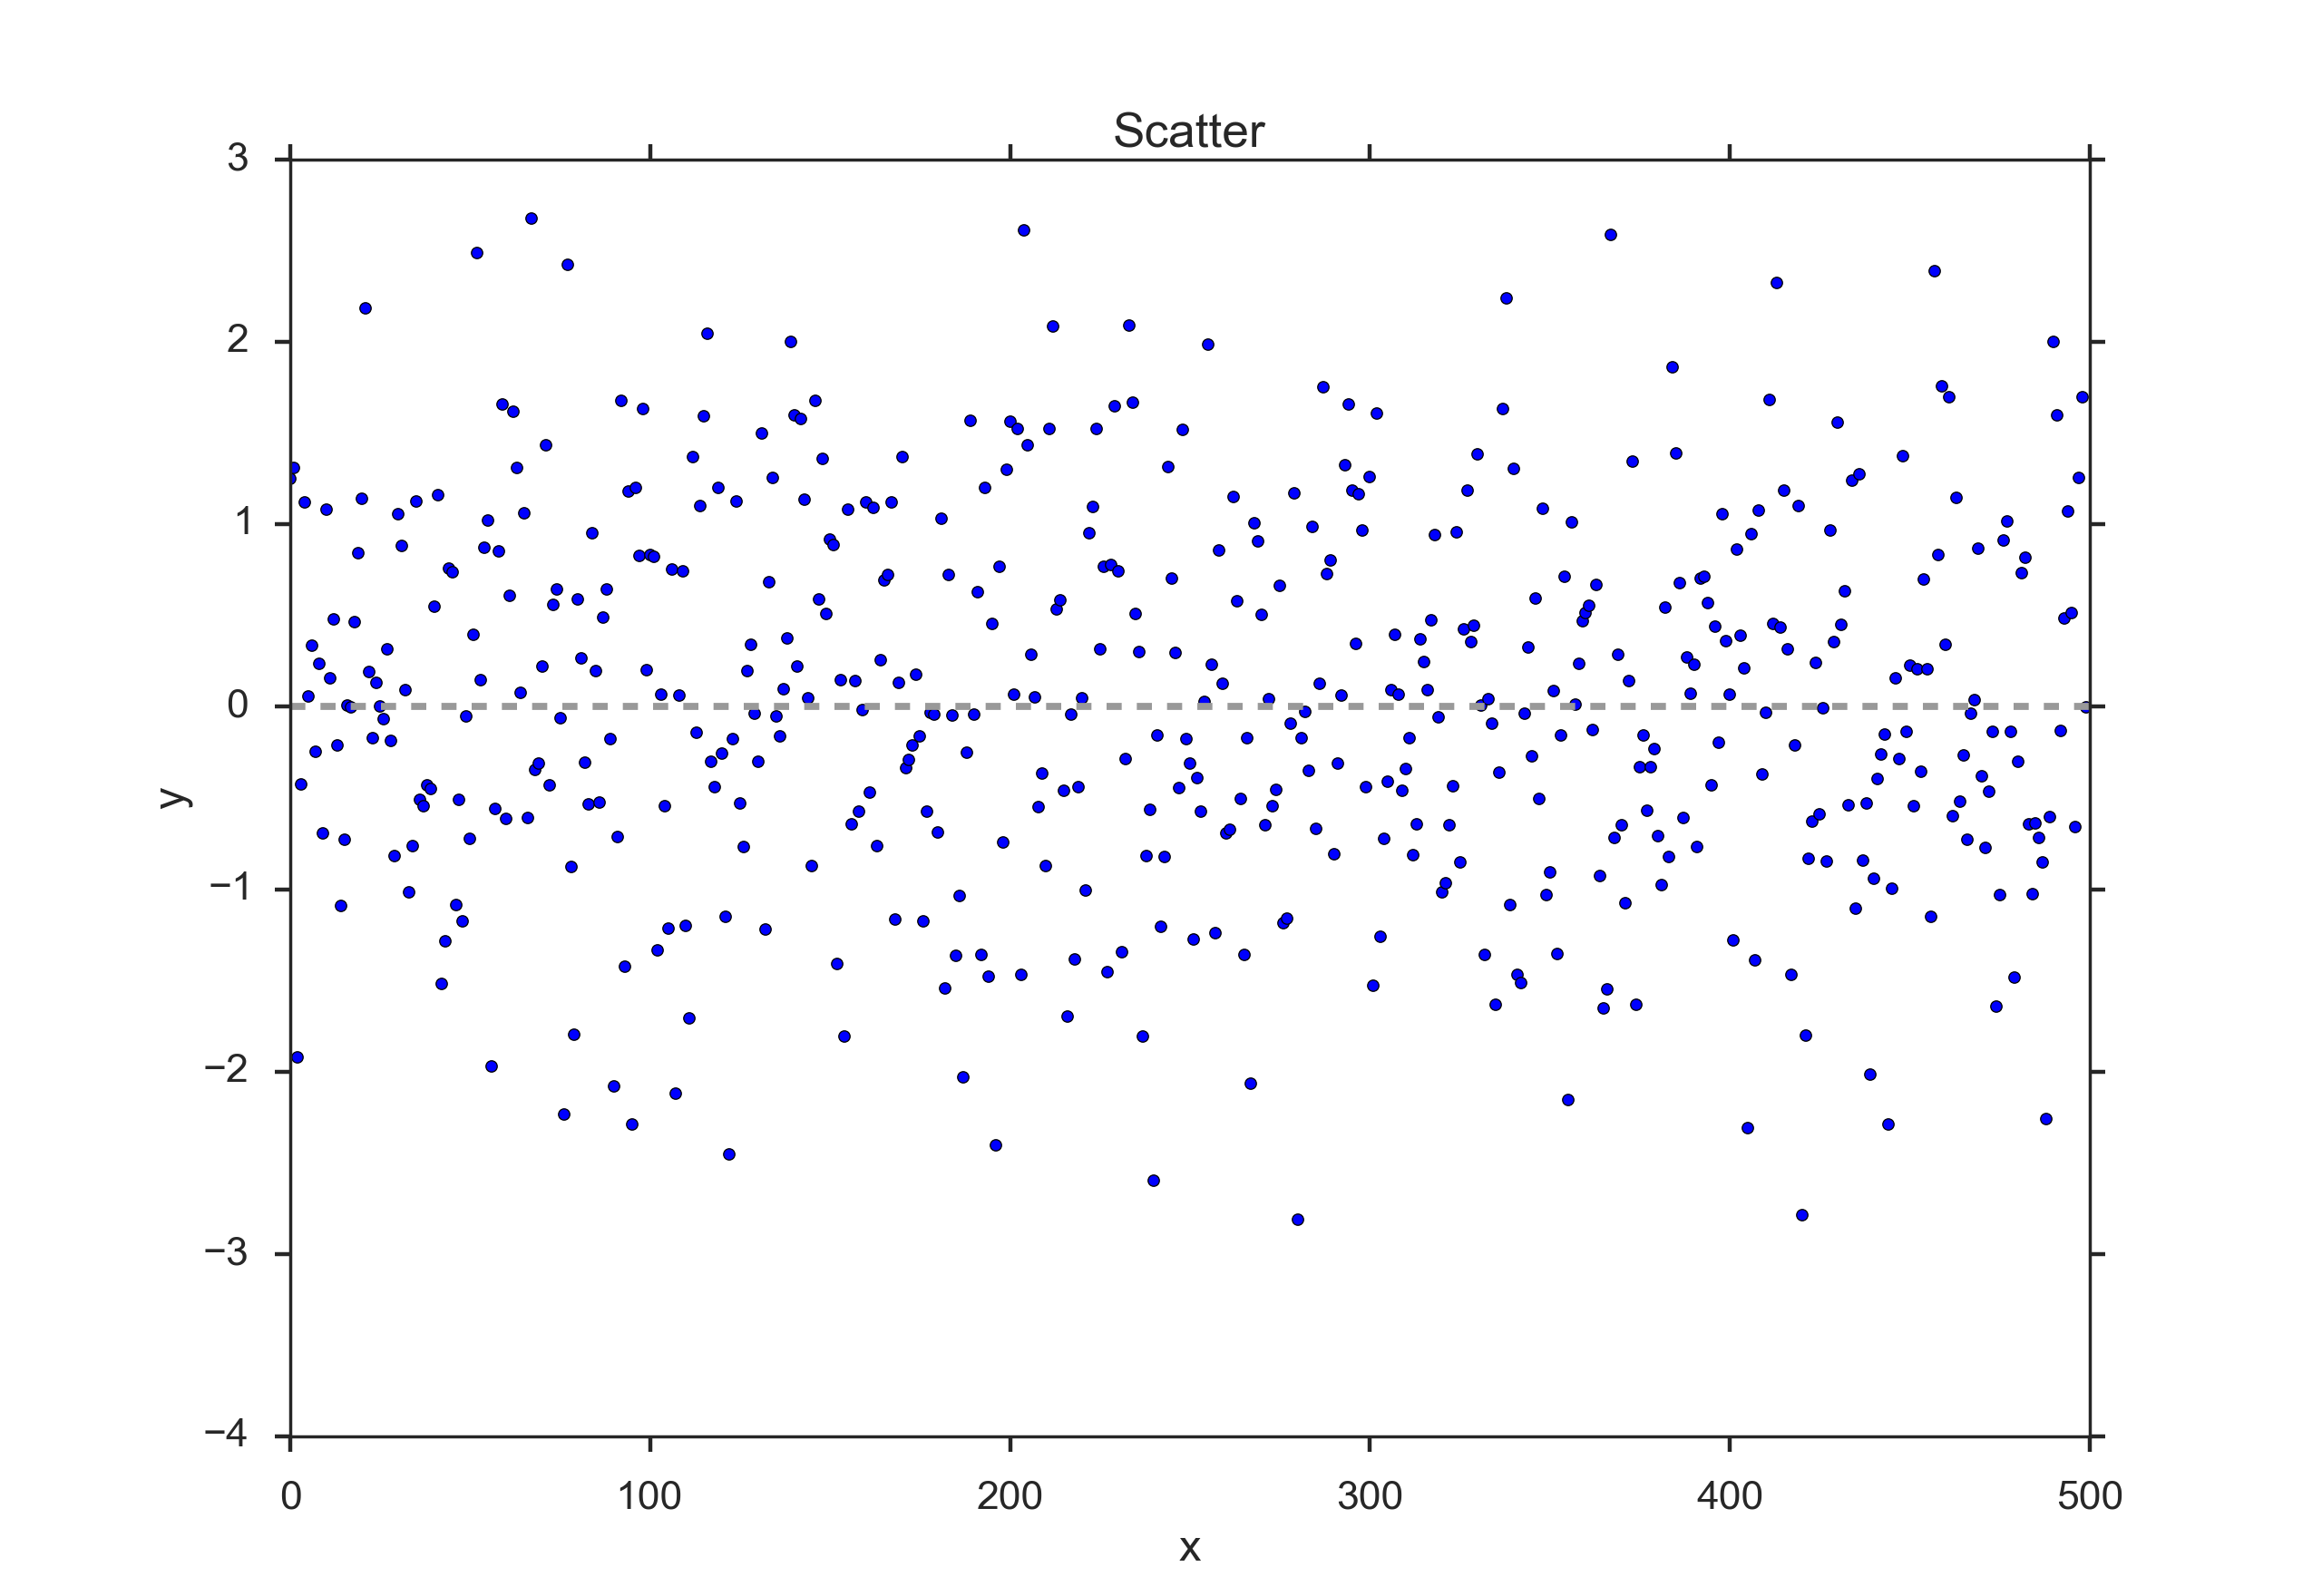
\includegraphics[width=0.5\textwidth]{../Images/scatterPlot.png}\\
  \caption{Scatter plot}
\end{figure}

\subsection{Histograms}\index{general}{plots!histogram}


\emph{Histograms} provide a first good overview of the distribution of your data.
If you divide by the overall number of data points, you get a \emph{relative frequency
histogram}; and if you just connect the top center points of each bin, you obtain a
\emph{relative frequency polygon}.

You can also smooth histograms with \emph{kernel-density-estimations (kde-plots)}. Those are nicely implemented and described in \emph{seaborn}.

\begin{figure}[ht]
  \centering
  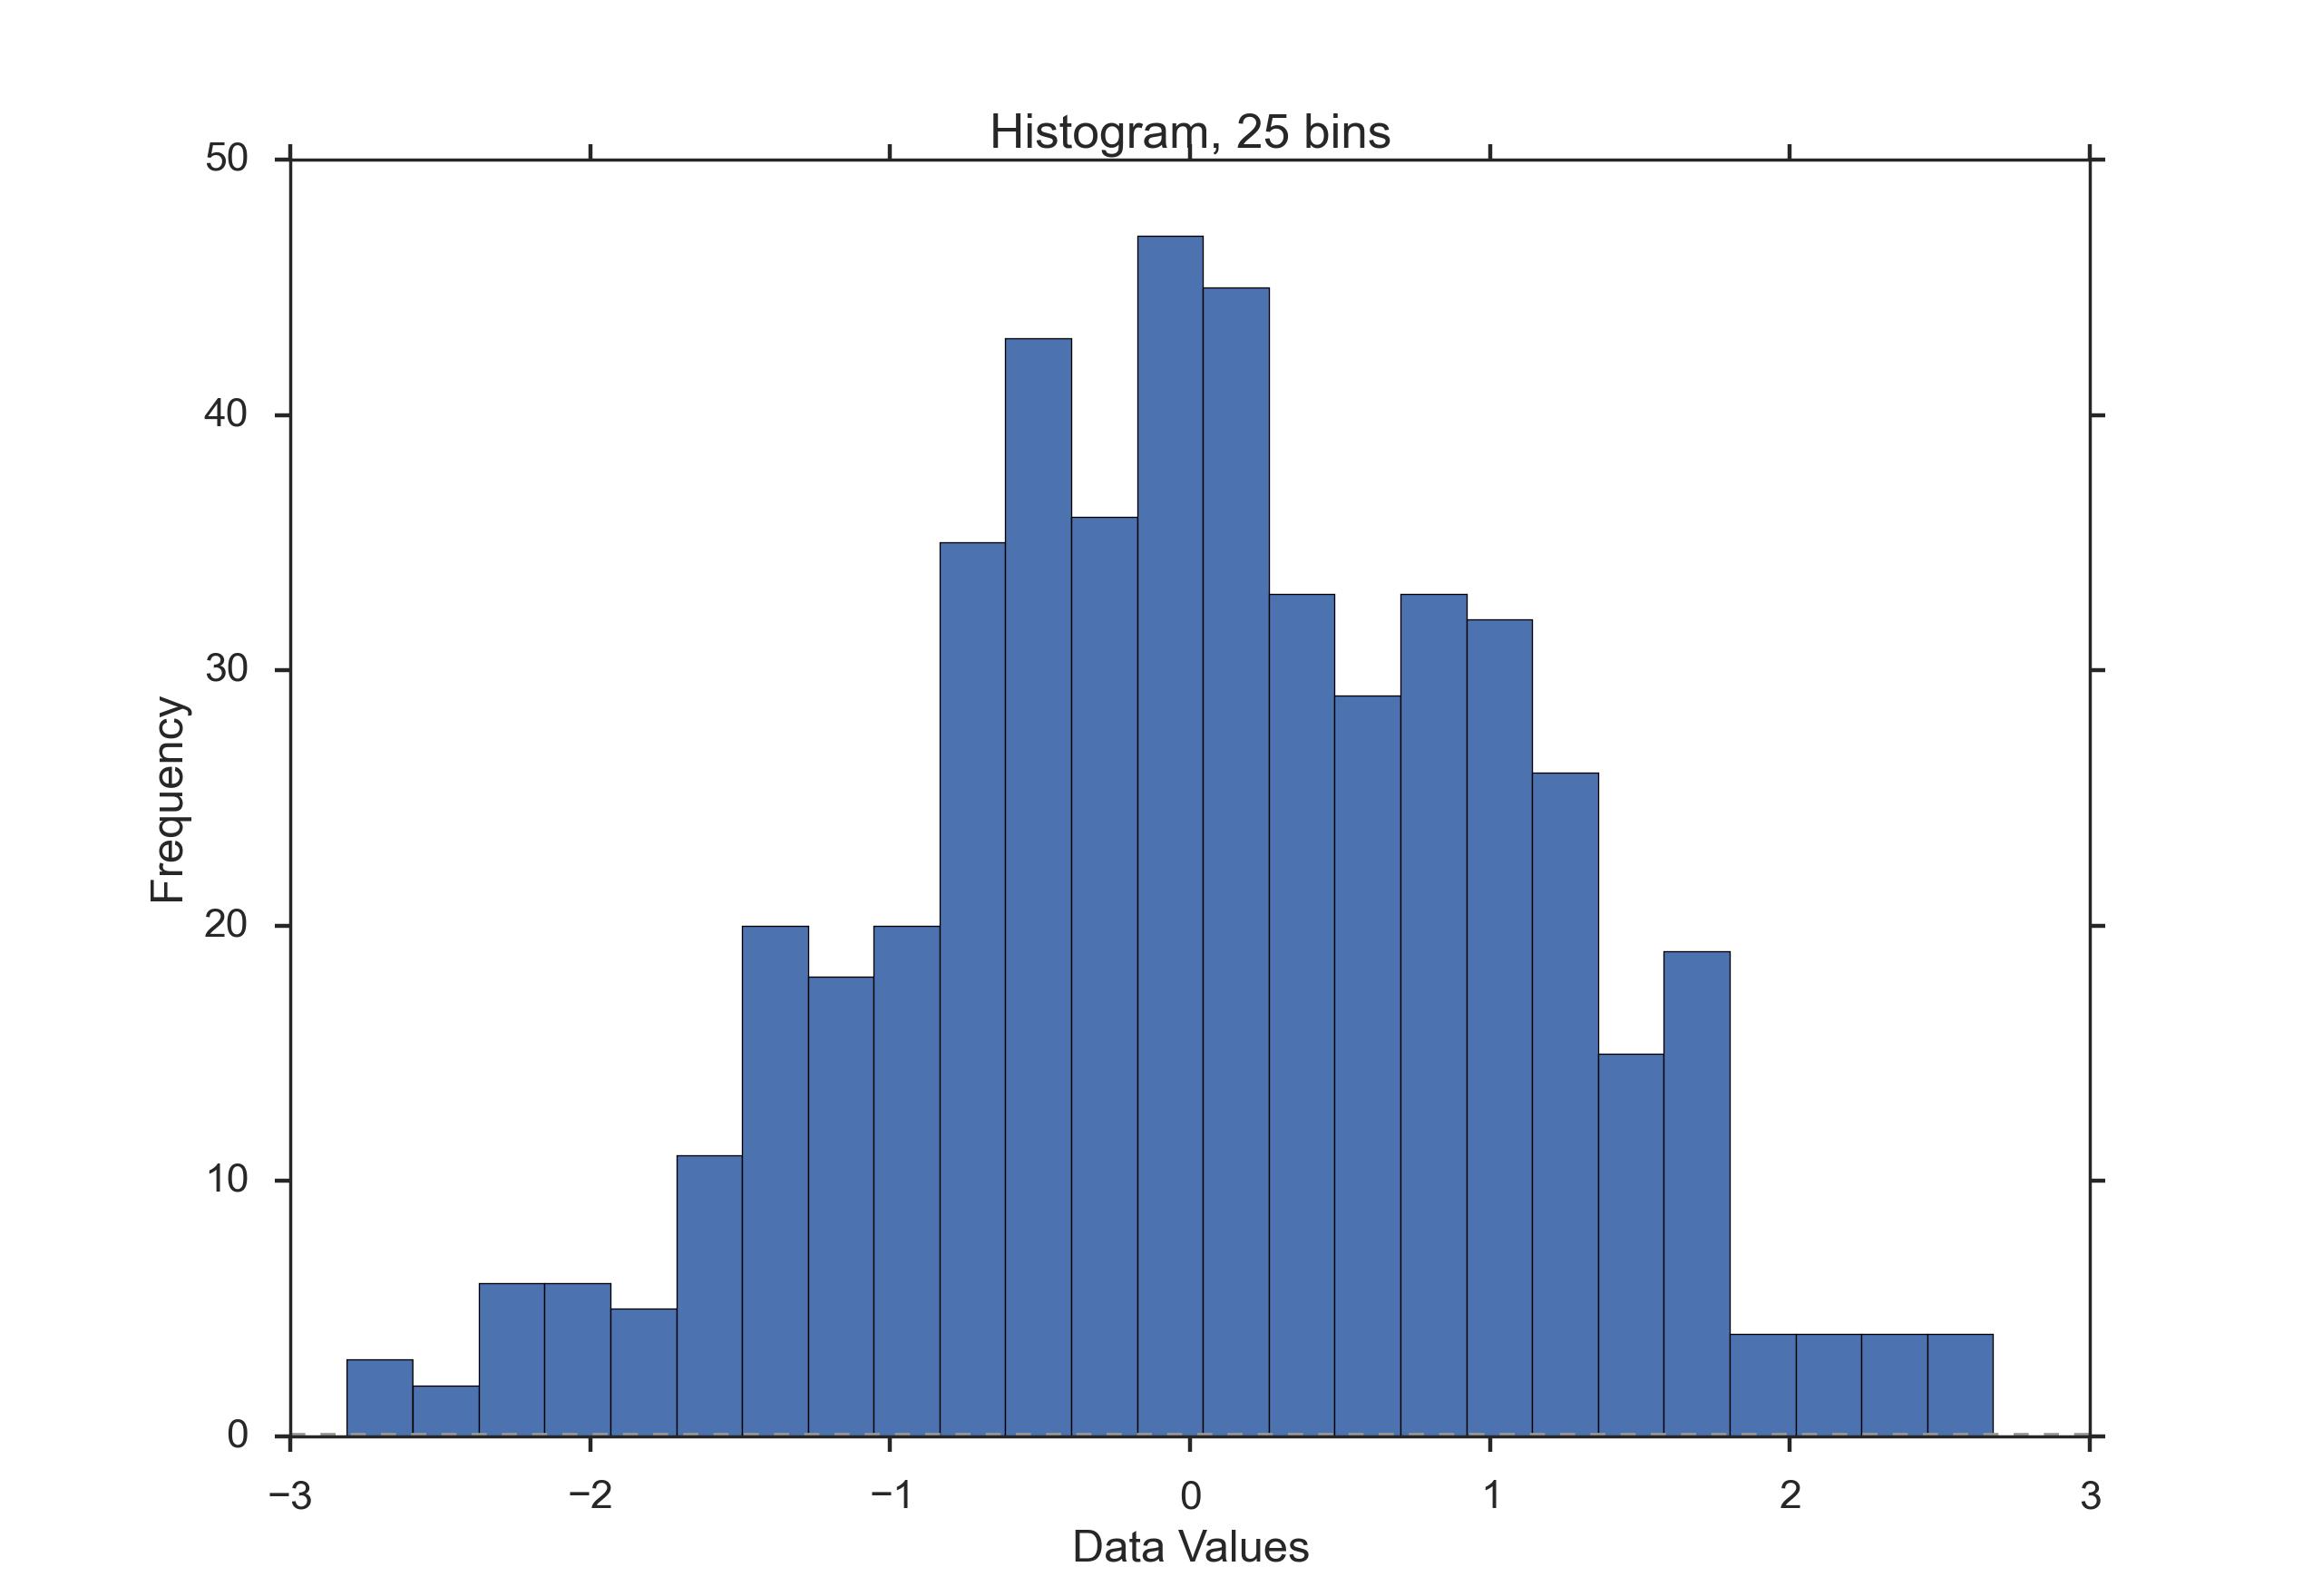
\includegraphics[width=0.5\textwidth]{../Images/Histogram.png}\\
  \caption{Histogram}
\end{figure}

\subsection{KDE-plots}\index{general}{plots!kde}

Histograms have the disadvantage that they are discontinuous, and that their shape critically depends on the chosen bin-width. In order to obtain smooth \emph{probability densities}, i.e. curves describing the likelihood of finding an event in any given interval, the technique of \emph{Kernel Density Estimation (KDE)}\index{general}{Kernel Density Estimator (KDE)} can be used. Thereby a normal distribution is typically used for the kernel. The width of this kernel function determines the amount of smoothing. To see how this works, we compare the construction of histogram and kernel density estimators, using these 6 data points: x = [−2.1, −1.3, −0.4, 1.9, 5.1, 6.2]. For the histogram, first the horizontal axis is divided into sub-intervals or bins which cover the range of the data. In this case, we have 6 bins each of width 2. Whenever a data point falls inside this interval, we place a box of height 1/12. If more than one data point falls inside the same bin, we stack the boxes on top of each other.

For the kernel density estimate, we place a normal kernel with variance 2.25 (indicated by the red dashed lines) on each of the data points xi. The kernels are summed to make the kernel density estimate (solid blue curve). The smoothness of the kernel density estimate is evident. Compared to the discreteness of the histogram, the kernel density estimates converge faster to the true underlying density for continuous random variables.

\begin{figure}[ht]
  \centering
  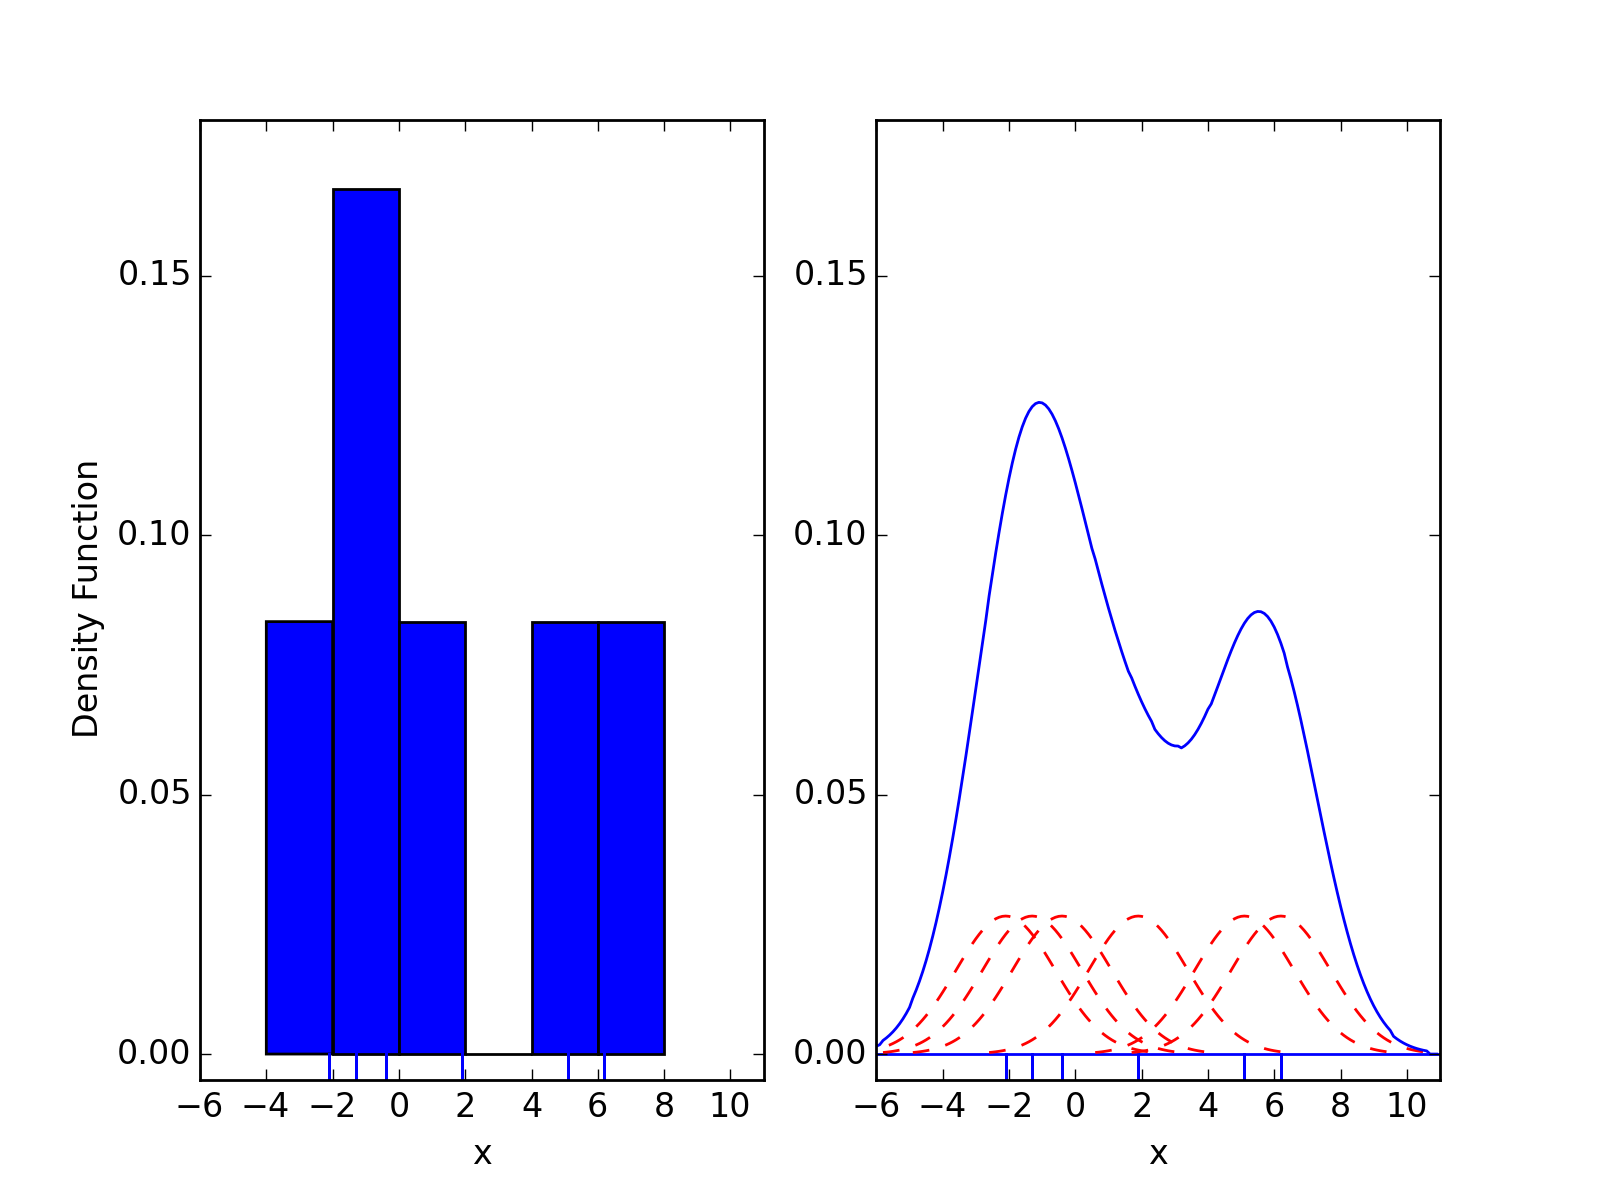
\includegraphics[width=0.75\textwidth]{../Images/KDEexplained.png}\\
  \caption{Comparison of the histogram (left) and kernel density estimate (right) constructed using the same data. The 6 individual kernels are the red dashed curves, the kernel density estimate the blue curves. The data points are the rug plot on the horizontal axis.}
\end{figure}


The bandwidth of the kernel is the parameter which determines how much we smooth out the contribution from each event. To illustrate its effect, we take a simulated random sample from the standard normal distribution, plotted as the blue spikes in the rug plot on the horizontal axis in Fig. \ref{fig:kdeBandwidth}, left. The right plot shows the true density (blue. a normal density with mean 0 and variance 1). In comparison, the gray dashed curve is undersmoothed since it contains too many spurious data artifacts arising from using a bandwidth h = 0.1 which is too small. The green dashed curve is oversmoothed since using the bandwidth h = 1 obscures much of the underlying structure. The red curve with a bandwidth of h = 0.42 is considered to be optimally smoothed since its density estimate is close to the true density.

\begin{figure}[ht]
  \centering
  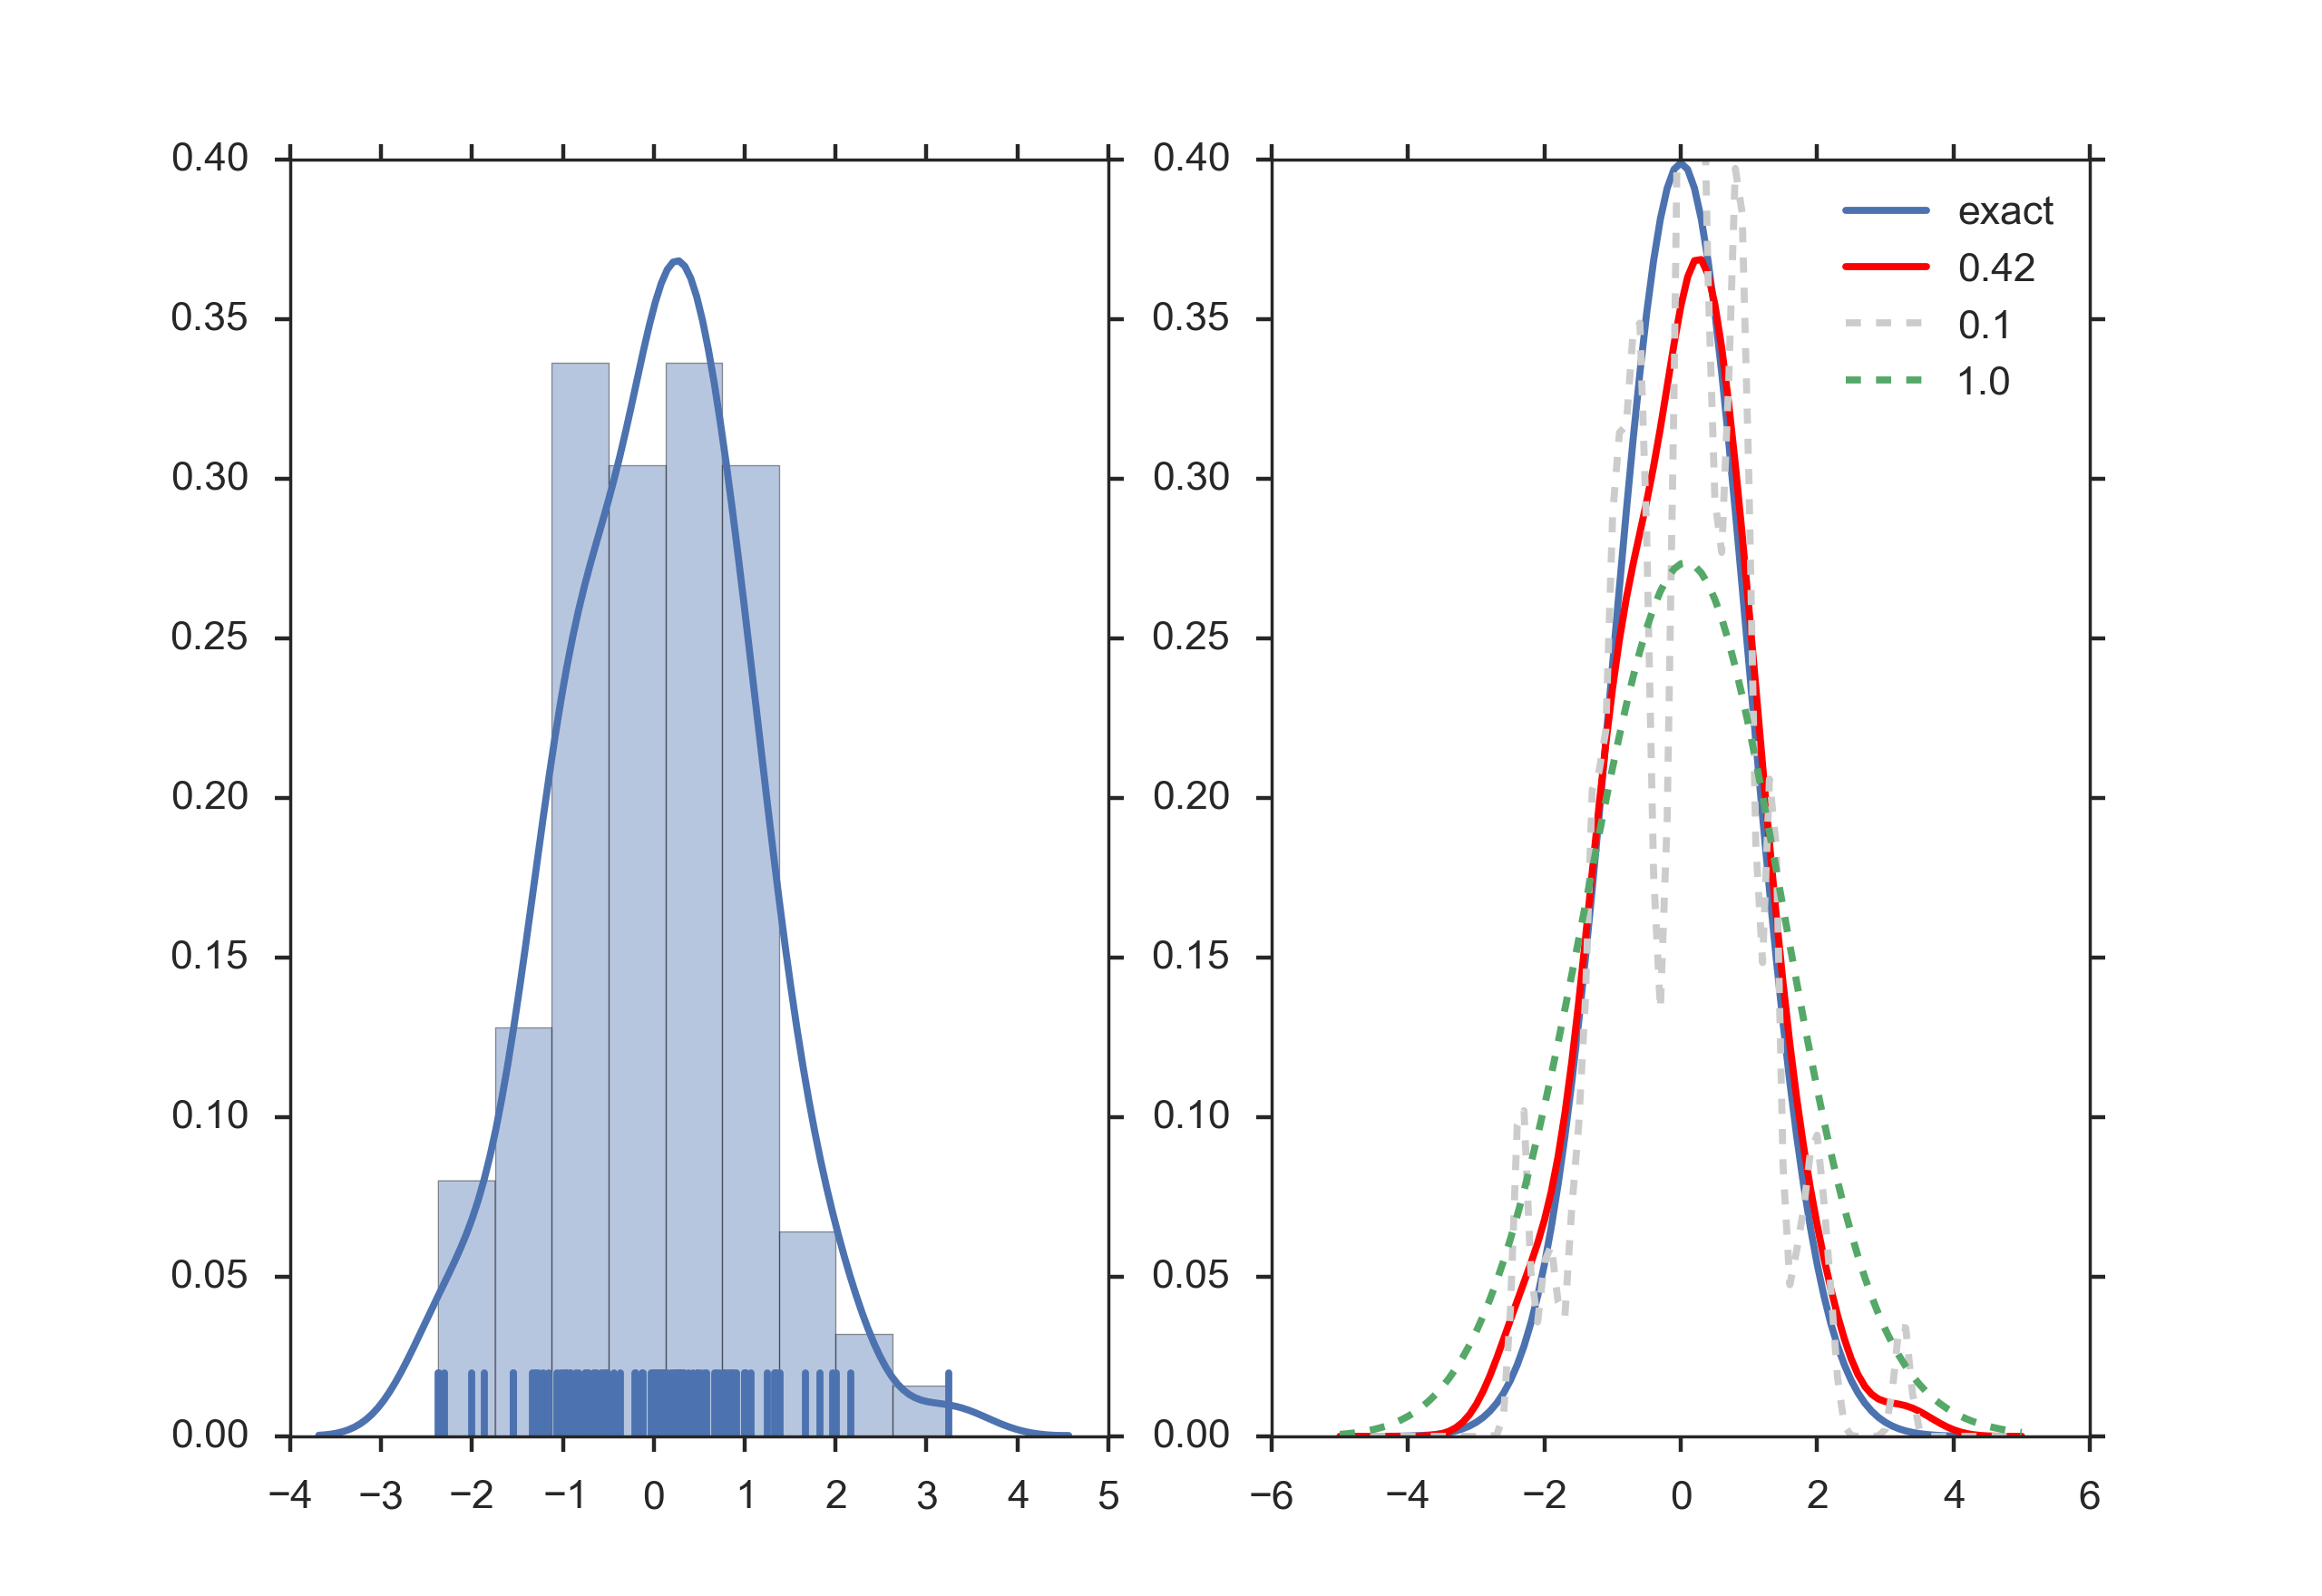
\includegraphics[width=0.75\textwidth]{../Images/KDEplot.png}\\
  \caption{ Left: Rug plot, histogram, and Kernel density estimate (KDE) of a random sample of 100 points from a standard normal distribution. Right: True density distribution (blue), and KDE with different bandwidths. Gray dashed: KDE with h=0.1; red: KDE with h=0.42 green dashed: KDE with h=1.0.}
  \label{fig:kdeBandwidth}
\end{figure}

It can be shown that under certain conditions the optimal choice for h is

\begin{equation}
  h = \left(\frac{4\hat{\sigma}^5}{3n}\right)^{\frac{1}{5}} \approx 1.06 \hat{\sigma} n^{-1/5},
\end{equation}

where $\hat{\sigma}$ is the standard deviation of the samples ("Silverman's rule of thumb").

\subsection{Cumulative Frequencies}\index{general}{cumulative frequency}

\emph{Cumulative frequency} curves indicate the number (or percent) of data with less than a given value. This is important for the statistical analysis (e.g. when we want to know the data range containing 95\% of all the values). Cumulative frequencies
are also useful for comparing the distribution of values in two or more different groups of individuals.

When you use percentage points, the cumulative frequency presentation has the additional advantage that it is bounded:

\begin{equation*}
  0 \leq x \leq 1
\end{equation*}

\begin{figure}[ht]
  \centering
  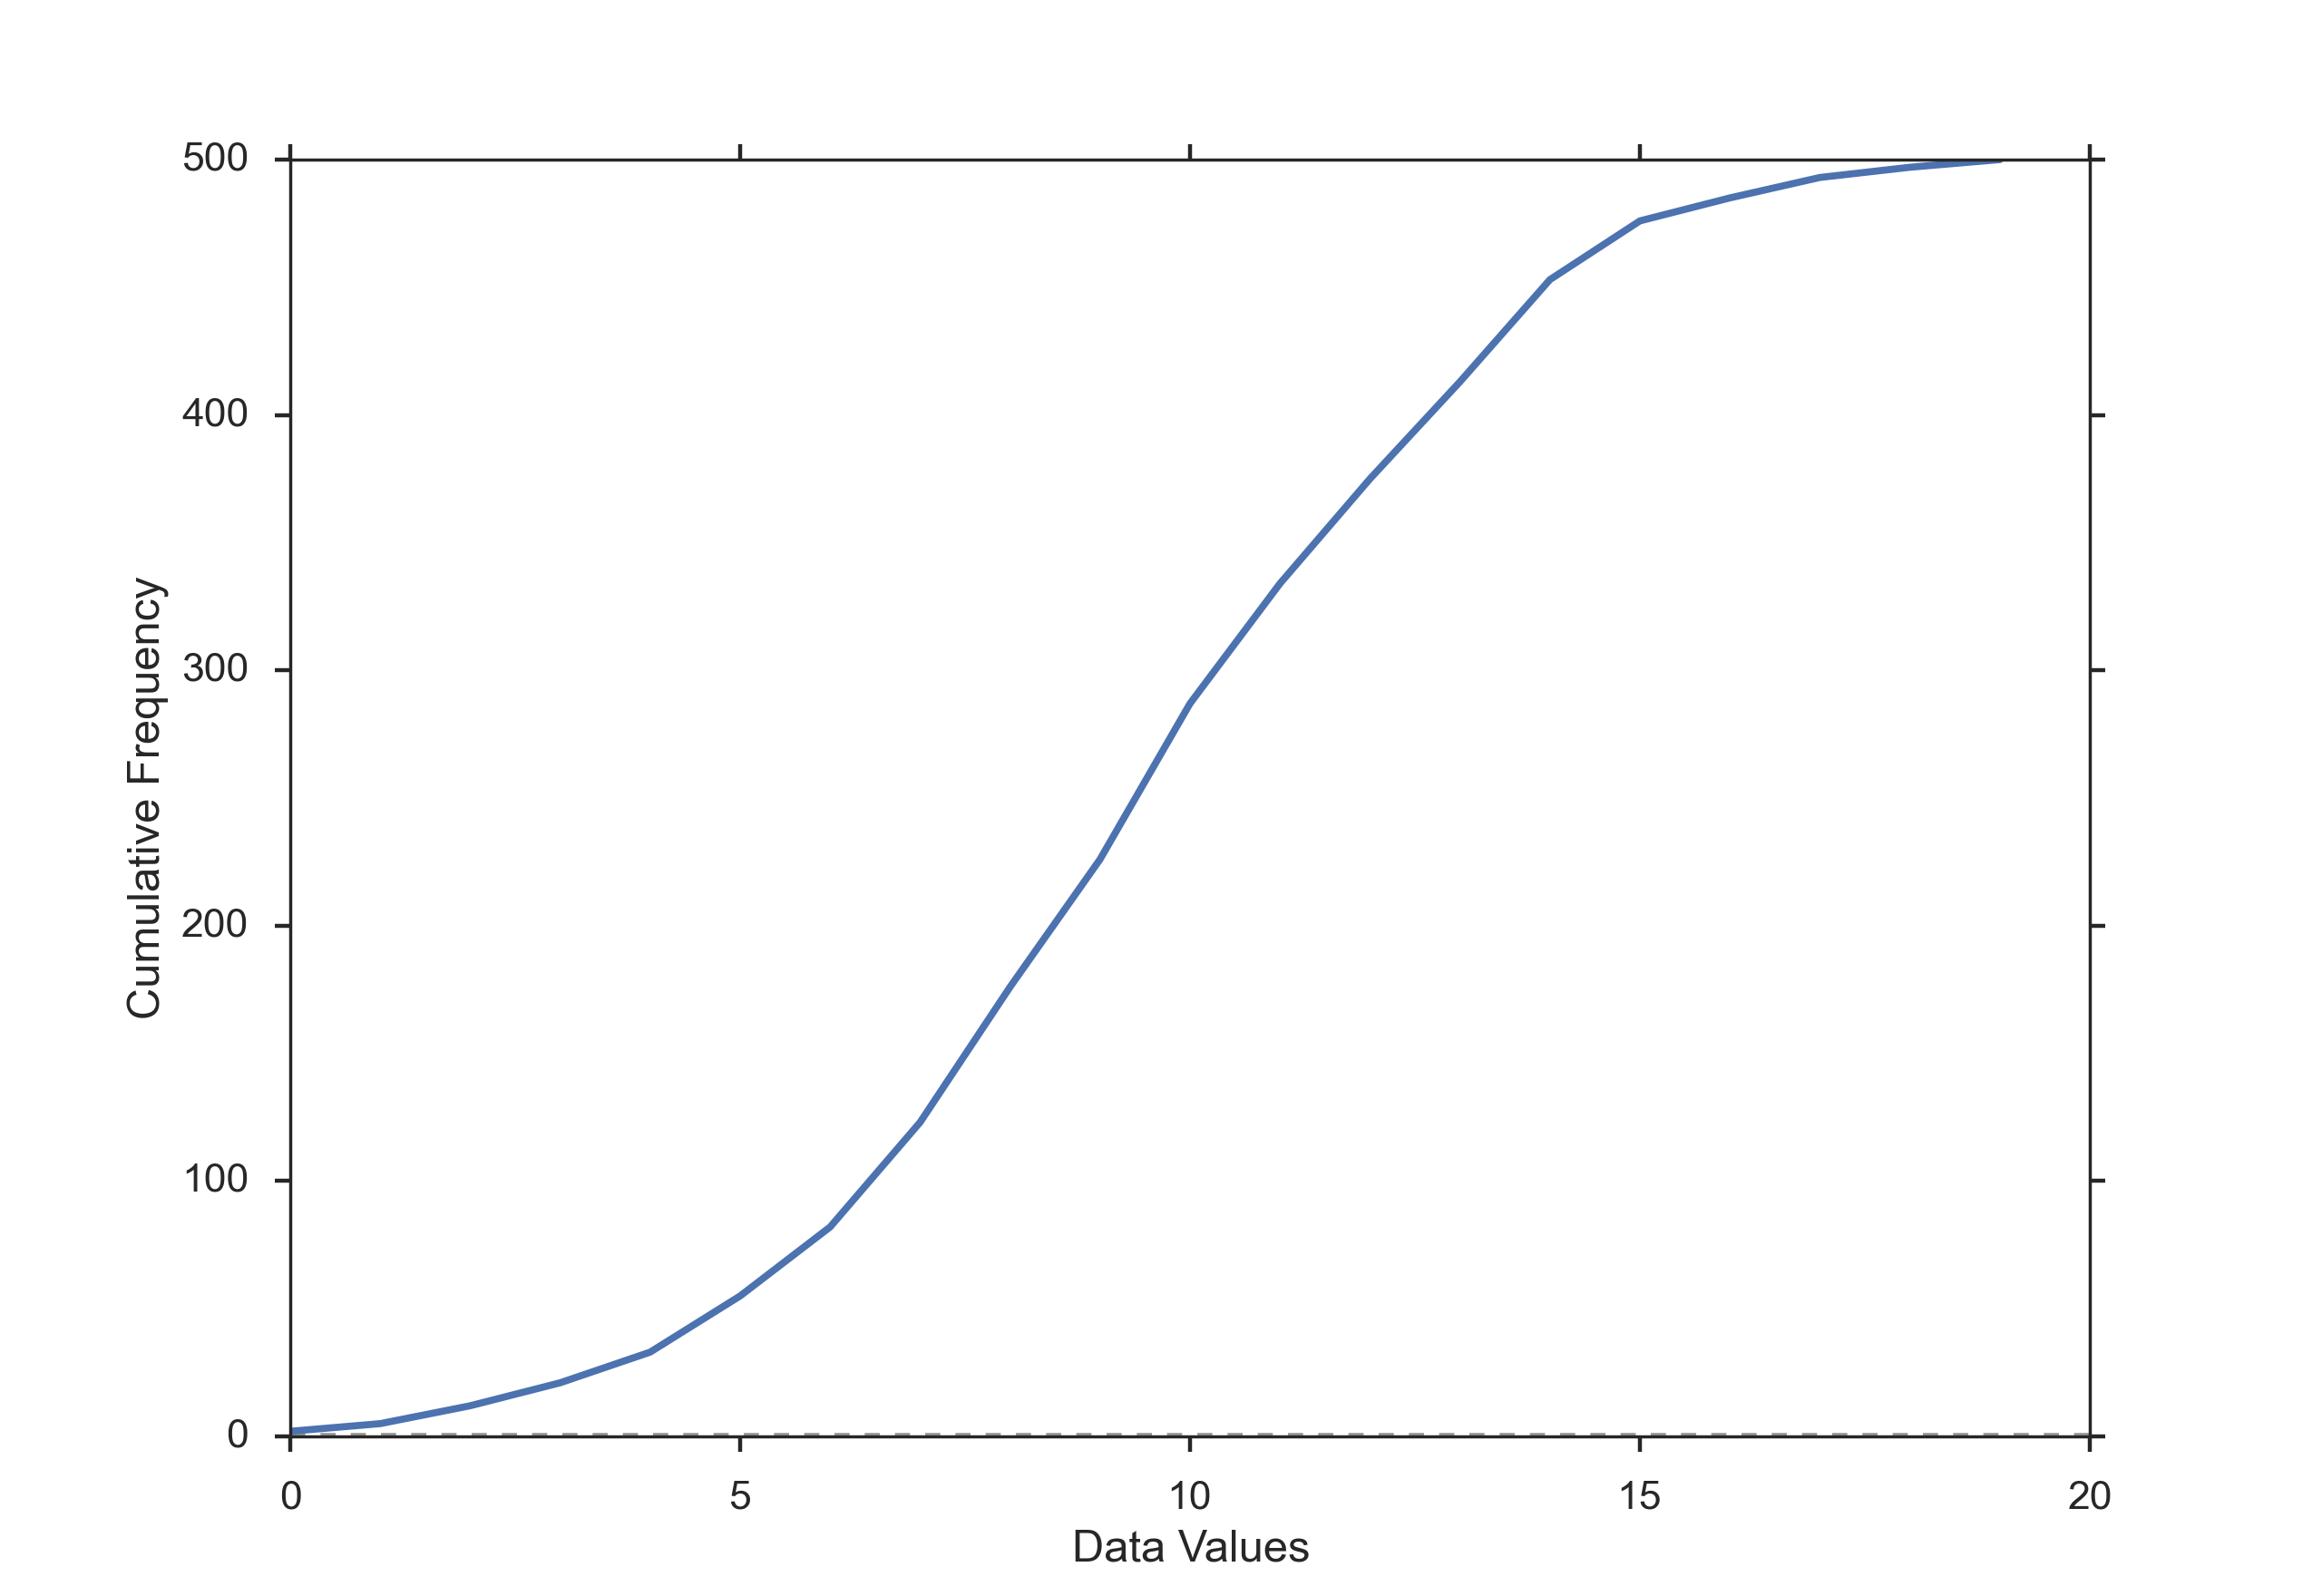
\includegraphics[width=0.5\textwidth]{../Images/CumulativeFrequencyFunction.png}\\
  \caption{Cumulative frequency function for a normal distribution.}
\end{figure}

\subsection{Errorbars}\index{general}{plots!errorbars}

\emph{Errorbars} are a common way to show mean value and variability when comparing a few measurement values. Note that you have to state explicitly if your errorbars correspond to the \emph{standard devation} or to the \emph{standard error} of the data. Using \emph{standard errors} has a nice feature: When error bars for the \emph{standard error} for two groups overlap, you can be sure the difference between the two means is not statistically significant (P>0.05). Watch out, though, since the opposite is not always true!

\begin{figure}[ht]
  \centering
  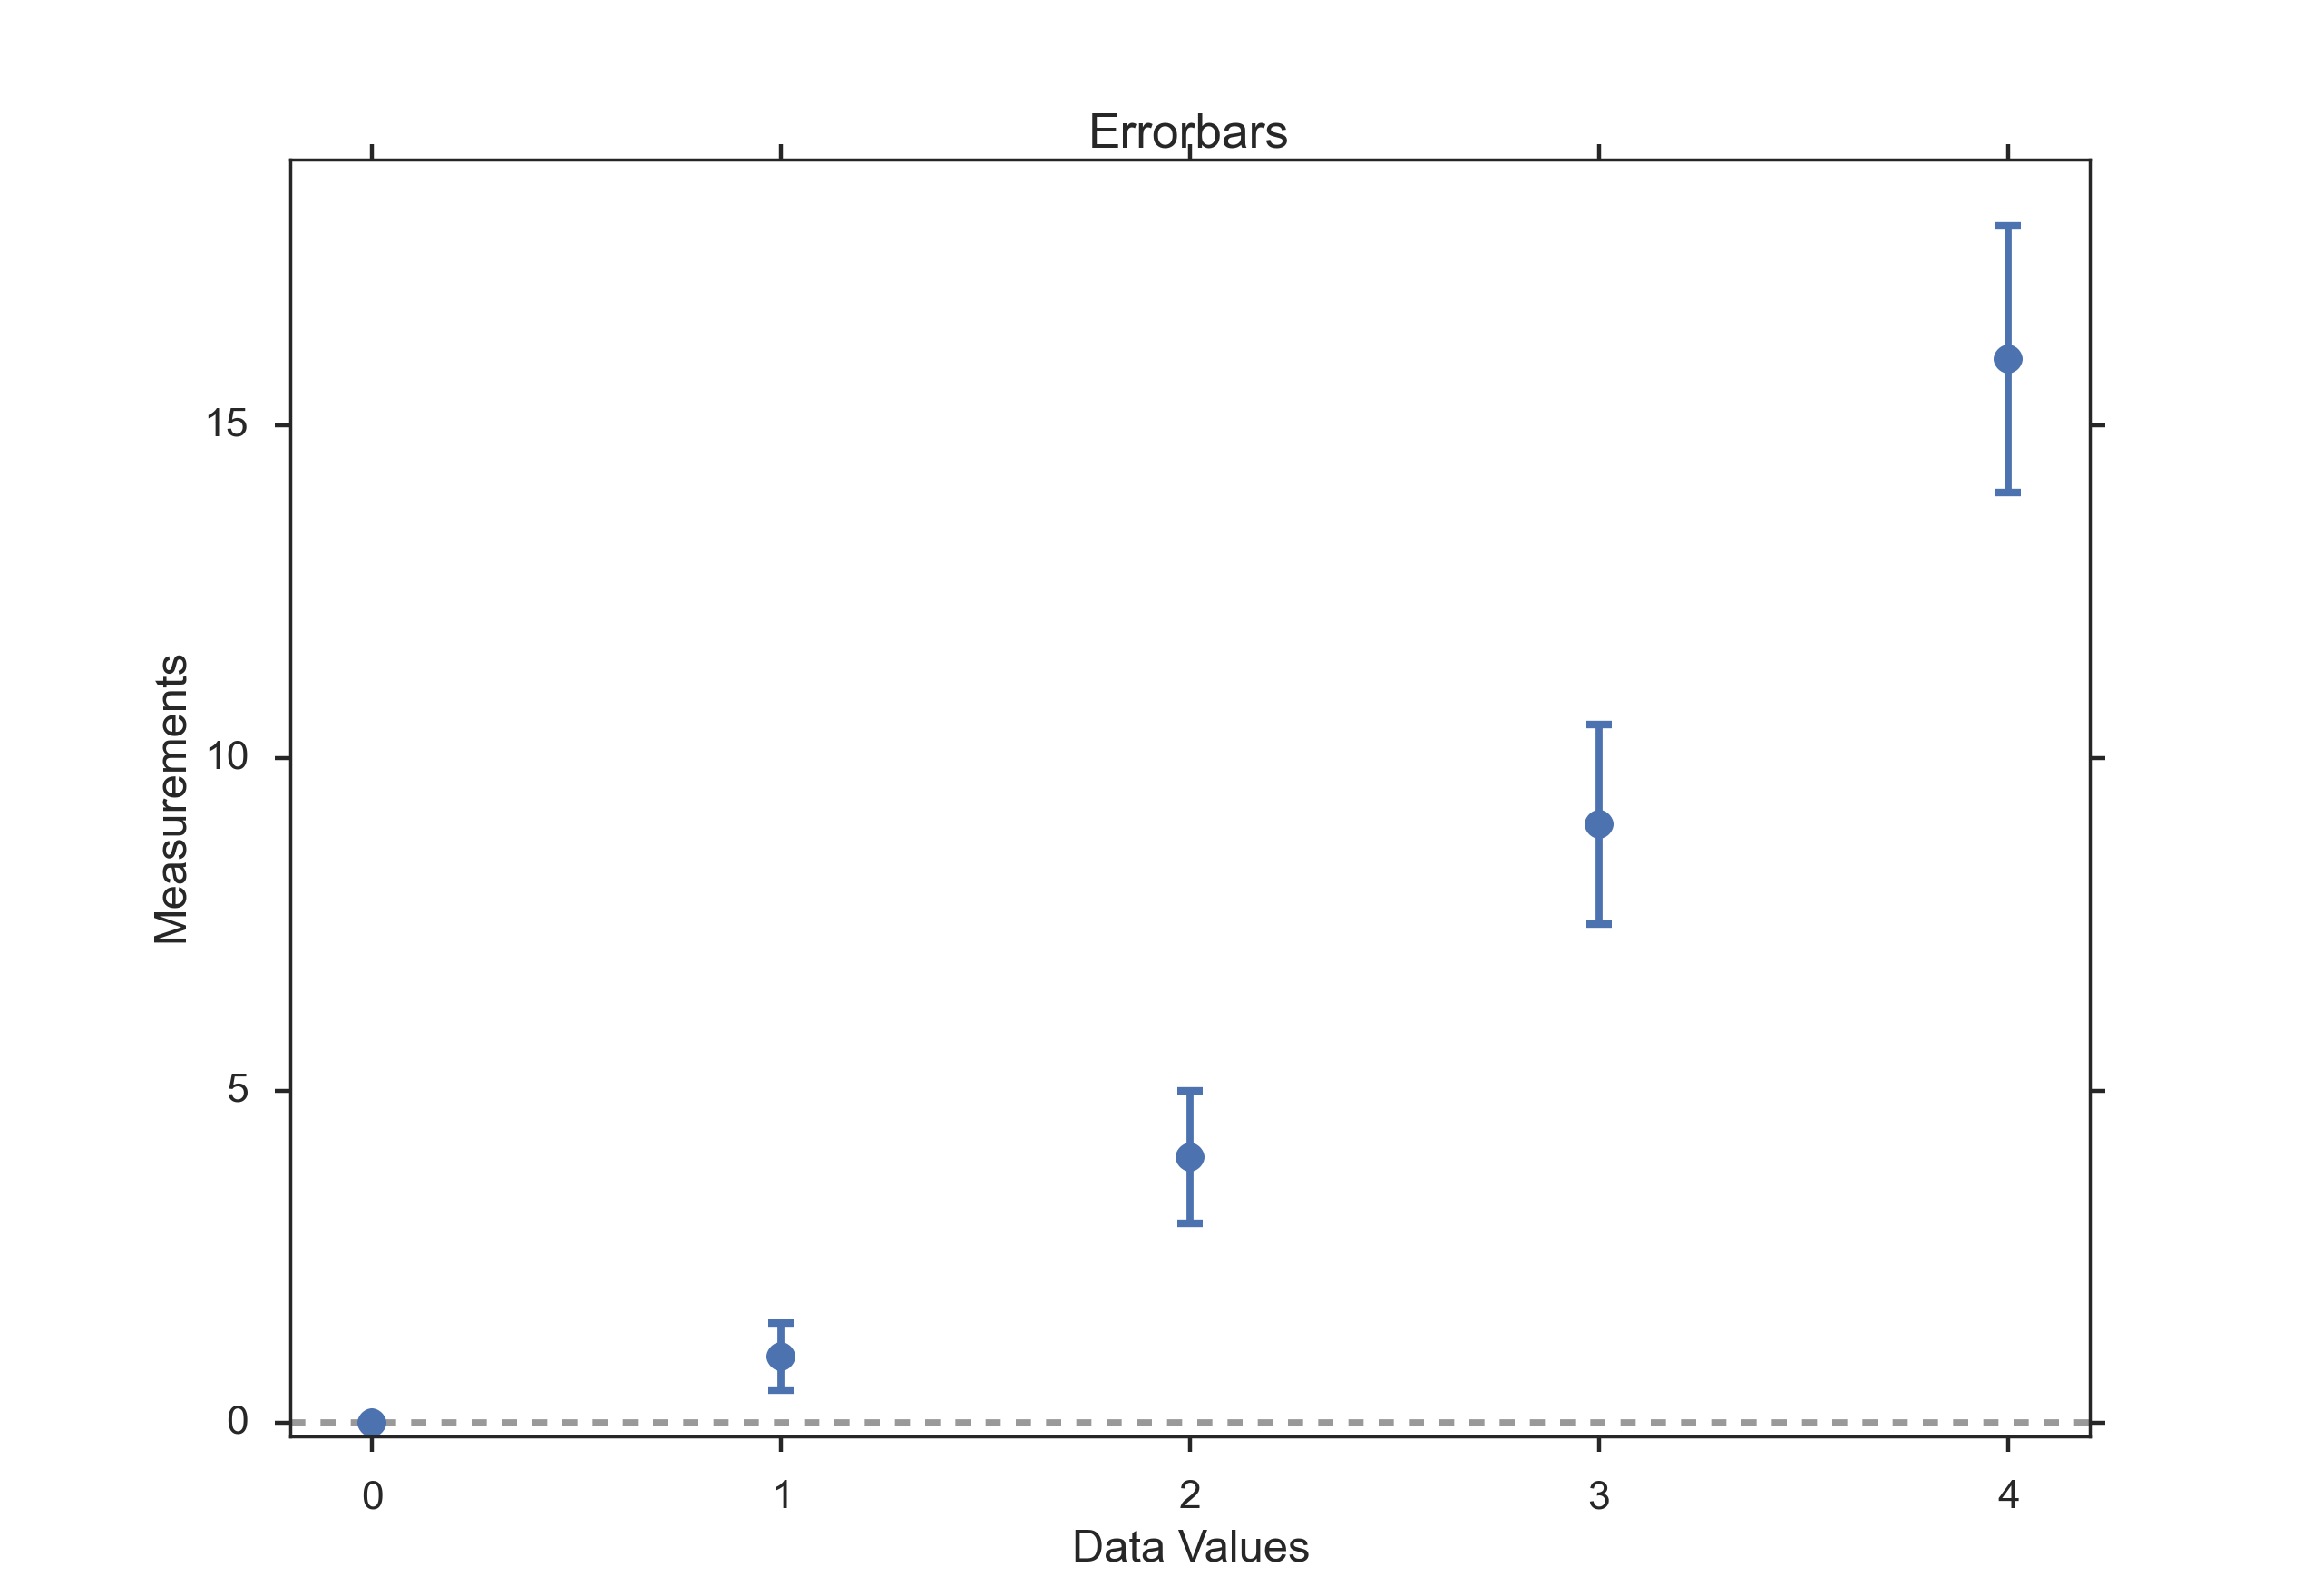
\includegraphics[width=0.5\textwidth]{../Images/Errorbars.png}\\
  \caption{Errorbars}
\end{figure}


\subsection{Box Plots}\index{general}{plots!boxplot}

\emph{Box plots} are frequently used in scientific publications to indicate values in two or more groups. The bottom and top of the box indicate the first and third quartiles, and the line inside the box shows the median. Care has to be taken with the whiskers, as different conventions exist for them. The most common form is that the lower whisker indicates the lowest value still within 1.5 \emph{inter-quartile-range} (IQR)\index{general}{inter-quartile-range, IQR} of the lower quartile, and the upper whisker the highest value still within 1.5 IQR of the upper quartile. Outliers (outside the whiskers) are plotted separately. Another convention is to have the whiskers indicate the full data range.

There are a number of tests to check for outliers\index{general}{outliers}. The method suggested by Tukey is to check for data which lie more than 1.5 * IQR above or below the first/third quartile (see Section \ref{sec:centiles}).

\begin{figure}[!ht]
  \centering
  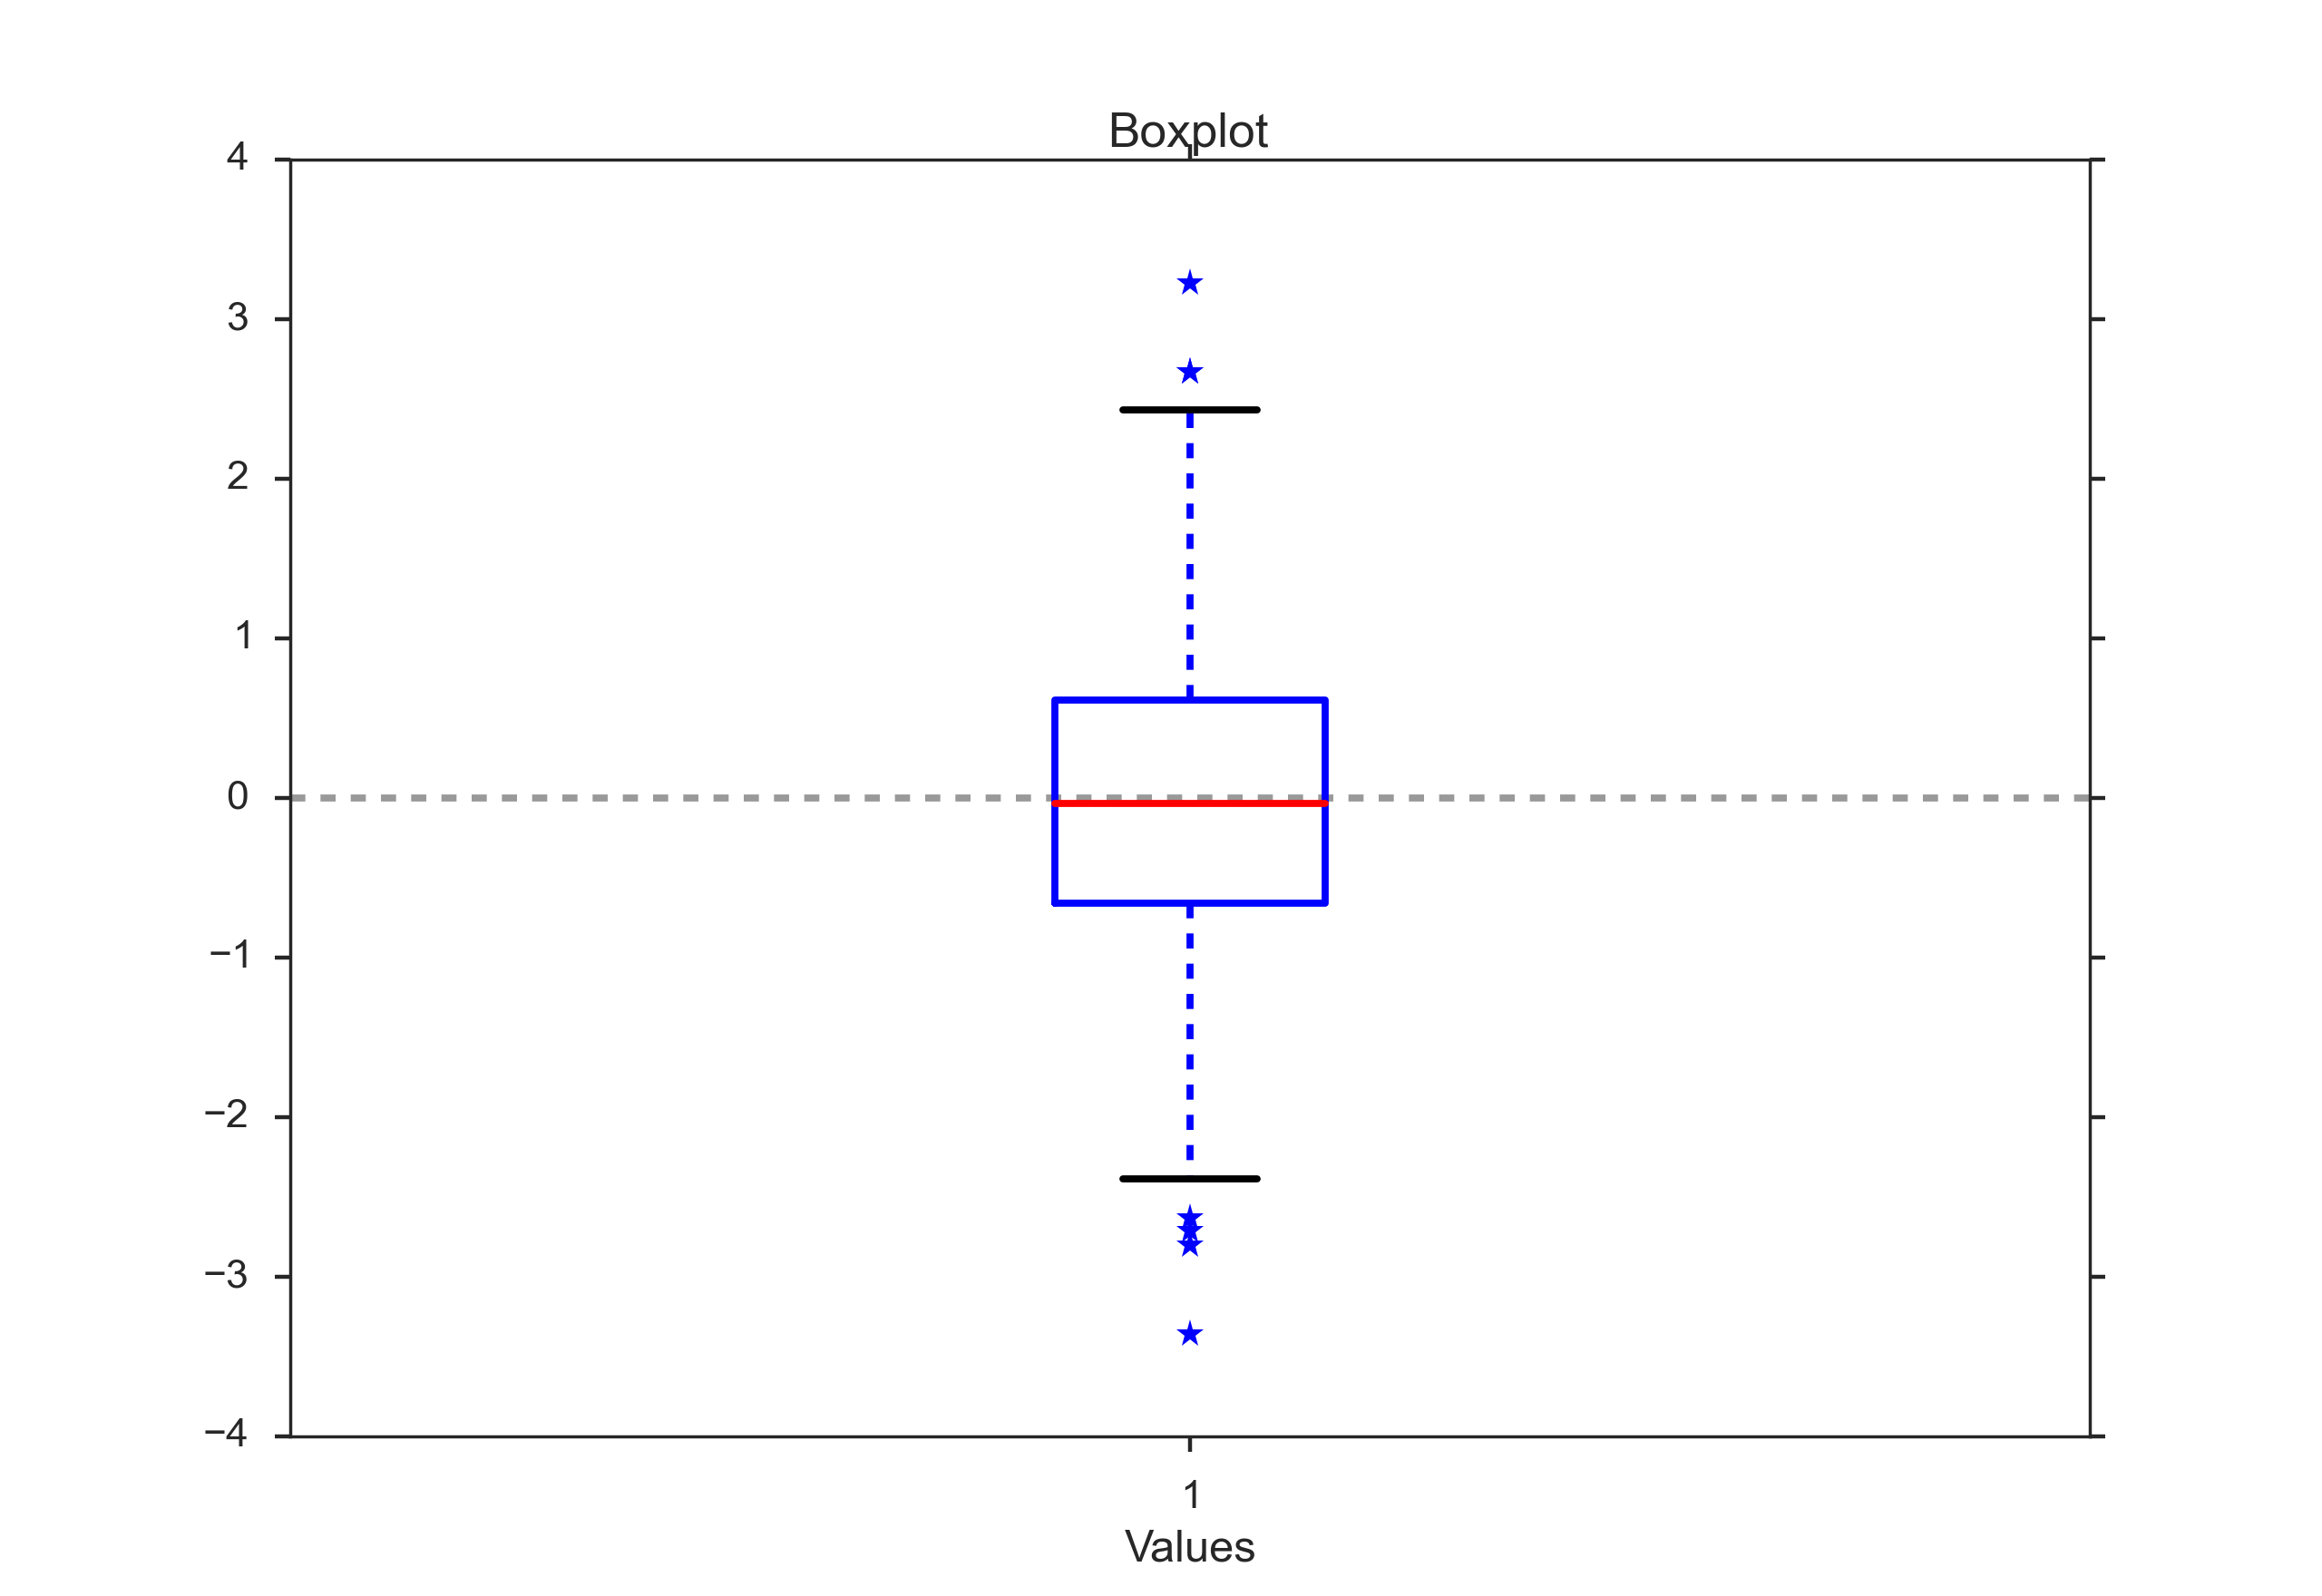
\includegraphics[width=0.5\textwidth]{../Images/boxplot.png}\\
  \caption{Box plot}\label{fig:Boxplot}
\end{figure}

Boxplots are often combined with KDE-plots to produce so-called \emph{violin-plots} \index {general}{plots!violinplot}, as shown in Figure \ref{fig:violin}.

\begin{figure}
  \centering
  % Requires \usepackage{graphicx}
  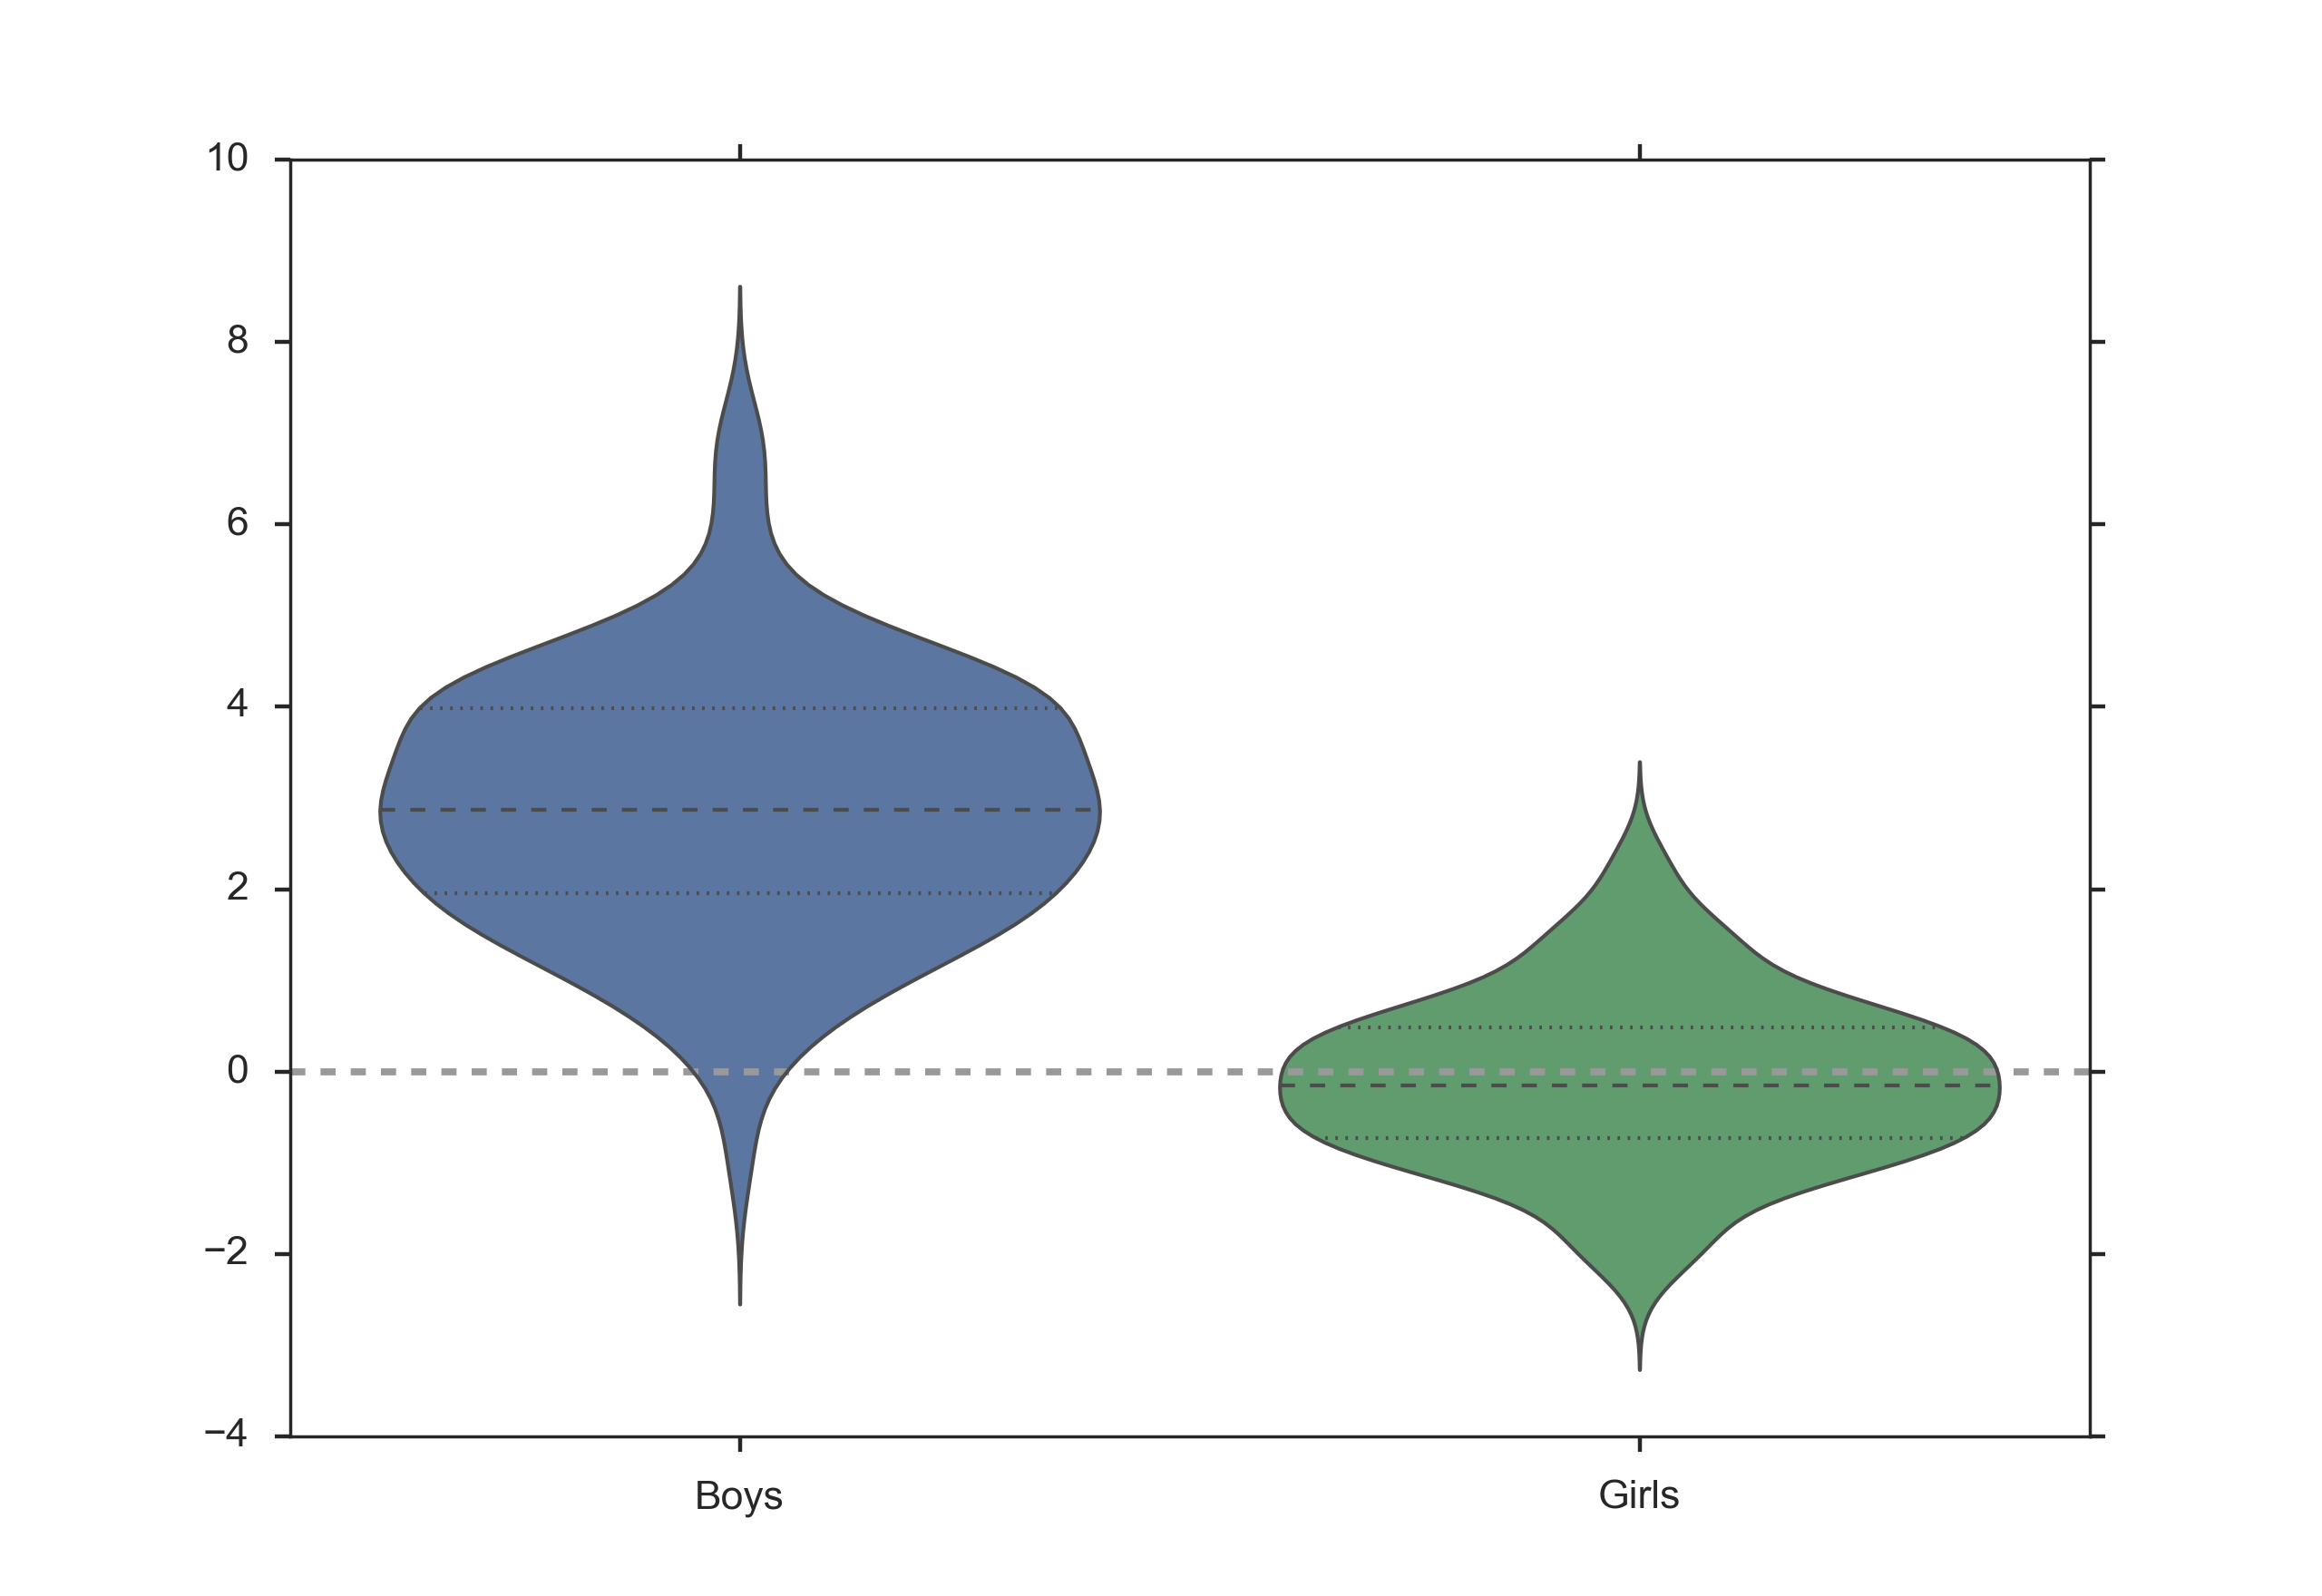
\includegraphics[width=0.75\textwidth]{../Images/violinplot.png}\\
  \caption{Violinplot, produced with \emph{seaborn}.}\label{fig:violin}
\end{figure}

\subsection{Programs: Data Display}
\PyImg "figsBasicPrinciples.py" (p \pageref{py:BasicPrinciples}) shows how the plots in this section have been generated.
\index{python}{figsBasicPrinciples}

\section{Populations and Samples}

The main difference between a \emph{population} and a \emph{sample} has to do with how observations are assigned to the data set (see Fig. \ref{fig:population}).

\begin{description}
  \item[Population] includes all of the elements from a set of data.
  \item[Sample] consists of one or more observations from the population.
\end{description}

\begin{figure}
  \centering
  % Requires \usepackage{graphicx}
  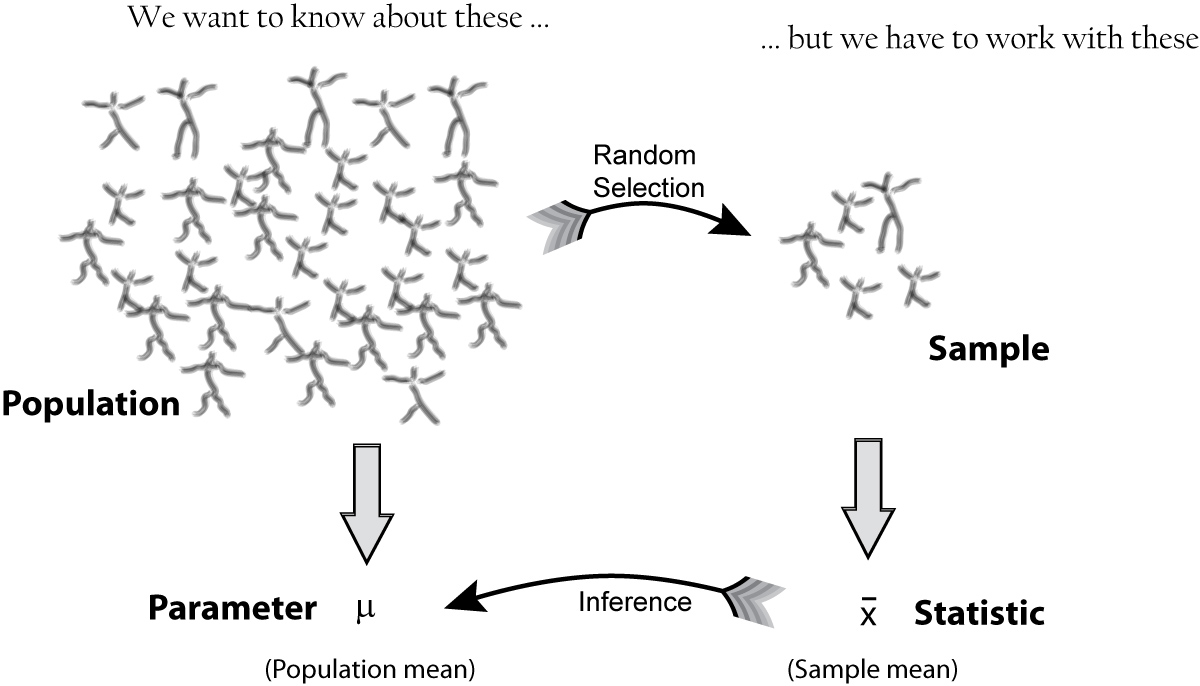
\includegraphics[width=1.0\textwidth]{../Images/PopulationAndSample.jpg}\\
  \caption{With statistical inference information from Samples is used to estimate Parameters from Populations.}\label{fig:population}
\end{figure}

More than one sample can be derived from the same population.

When estimating a \emph{parameter} of a \emph{population}, e.g. the weight of male Europeans, we can typically never measure all of them. We have to confine ourselves to investigate a (hopefully representative) random \emph{sample} of this group. Based on the \emph{sample statistic}, we use \emph{statistical inference} to find out what we know about the \emph{parameter}.

\begin{description}
  \item[Parameter] characteristic of a population, such as a mean or standard deviation. Often denoted with Greek symbols.
  \item[Statistic] a measurable characteristic of a sample.
  \item[Sampling distribution] is the probability distribution of a given statistic based on a random sample.
  \item[Statistical inference] enables you to make an educated guess about a population parameter based on a statistic computed from a sample randomly drawn from that population.
\end{description}

An example for parameters and statistics is given in Table \ref{table:population}.

\begin{table}[ht]

  \centering
    \begin{tabular}{|l|c|c|}
      \hline
       & Sample Statistic & Population Parameter \\
       \hline
      Mean & $\bar{x}$ & $\mu$ \\
      Standard Deviation & s & $\sigma$ \\
      \hline
    \end{tabular}
    \caption{Comparison of Sample Statistics and Population Parameters.}
    \label{table:population}
\end{table}


\section{Study Design}

\subsection{Terminology}

\begin{figure}
  \centering
  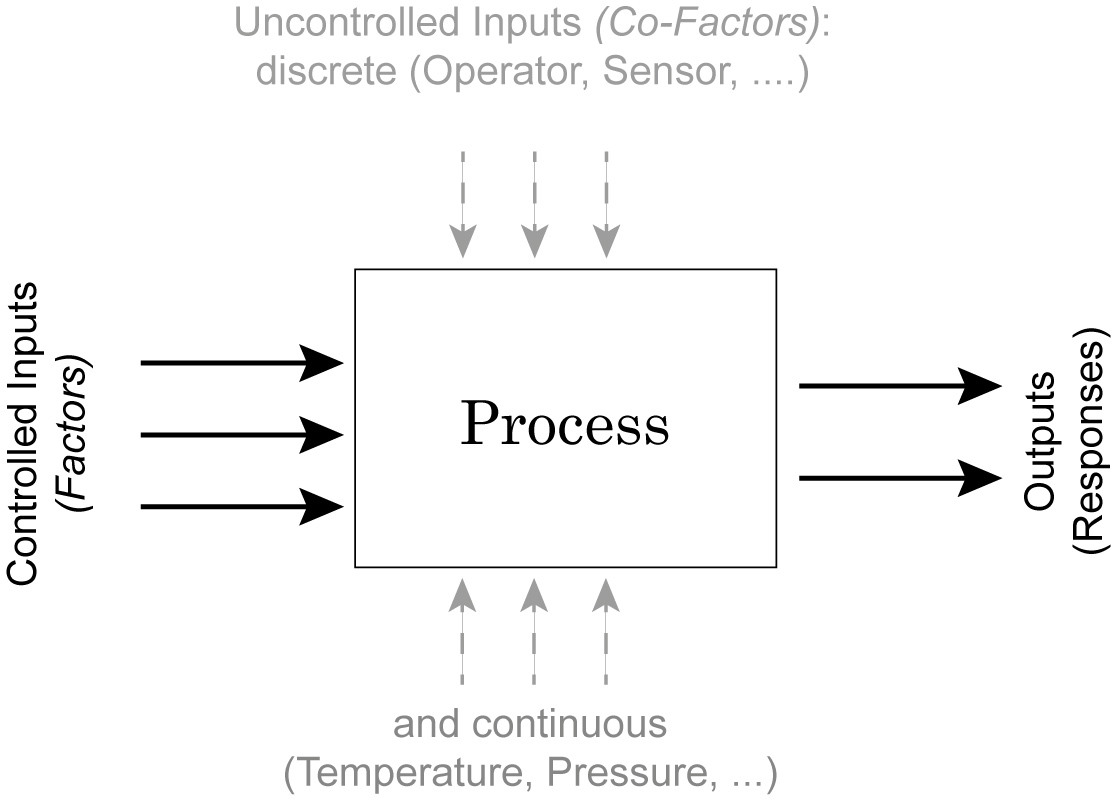
\includegraphics[width=0.75\textwidth]{../Images/Process_Optimization.jpg}\\
  \caption{Process Schematic}\label{fig:StudyDesign}
\end{figure}

In the context of study design, different terminologies can be found (Fig. \ref{fig:StudyDesign}):

\begin{itemize}
    \item{The controlled inputs are often called \emph{factors}\index{general}{factors} or
            \emph{treatments}\index{general}{treatments}.}
    \item{The uncontrolled inputs are called \emph{co-factors}\index{general}{co-factors} or
            \emph{nuisance factors}.}
\end{itemize}

When we try to model a process with two inputs and one outputs, we can
formulate a mathematical model for example as

\begin{equation}
    X = \beta_0 + \beta_1 X_1 + \beta_2 X_2 + \beta_{12} X_1 X_2 + \epsilon
\end{equation}

The terms with the single "X's" are called \emph{main effects}\index{general}{main effects}, and the terms with multiple "X's" \emph{interaction terms}\index{general}{interactions}. And since the $\beta$
parameters enter the equation only linearly, this is referred to as a \emph{general linear model}. The $\epsilon$s are called \emph{residuals}, and
are expected to be approximately normally distributed around zero.

\subsection{Overview}

The first question you have to ask yourself is what you want to do. Do you want to

\begin{itemize}
    \item{Compare two or more groups, or one group to a fixed value?}
    \item{Screen the observed responses to identify
            factors/effects that are important?}
    \item{Maximize or minimize a response (variability, distanct to target,
            robustness)?, or}
    \item{Develop a regression model to quantify the dependence of a
            response variable on the process input?}
\end{itemize}

The first question leads to an hypothesis test. The second one is a screening investigation, where you have to watch out for \emph{multiple testing artefacts}. The third task is an optimization problem. And the last one brings you into the realm of \emph{statistical modeling}.

Once you have determined \emph{what} you want to do, you have to decide \emph{how} you want to do this. You can either do \emph{controlled experiments}. Or you can use \emph{observations} to obtain the data that you are looking for. In a controlled experiment you typically try to vary only a single parameter, and investigate the effects of that parameter on the output.

\subsection{Personal Tips}

\begin{enumerate}
  \item Be realistic about your task.
  \item Plan in sufficient control/calibration experiments.
  \item Take notes.
  \item Store your data in a well structured way.
\end{enumerate}

\subsubsection{Preliminary Investigations and Murphy's Law}
Most investigations require more than one round of experiments and analyses. The theory goes that you first state your hypothesis, then do the experiments, and accept or reject the hypothesis. Done.
Most of my investigations have been less straightforward. Typically, you start out with an idea. After making sure that nobody else has solved your question before, you sit down and do the first rounds of measurements, and write the analysis programs required to analyze your data. Thereby you find most of the things that can go wrong (they typically do, as indicated by \emph{Murphy's Law}), and what you should have done differently in the first place. Not only does that first round of investigation provide a \emph{proof of principle} that your question is tractable, but you also have obtained some data on the variability of typical responses. This allows you to obtain a reasonable estimate of the number of subjects/samples you need in order to accept or reject your hypothesis. By this time you also know if your experimental setup is sufficient, or if you need a higher quality measurement equipment. The second round of investigations is in most cases the real stuff, and (hopefully) provides you with enough data to publish your findings.

\subsubsection{Calibration Runs}
If anyhow possible, you should start out and end your recordings with something that you know. For example during movement recordings I try to start out with recording a stationary point, and then move it 10 cm forward, left, and up. Having a recording where you know exactly what happens not only helps to detect drift in the sensors, and problems in the experimental setup. These recordings also help to verify the accuracy of your analysis programs.

\subsubsection{Documentation} \index{general}{documentation}
Make sure that you document all the factors that may influence your results, and everything that happens during the experiment:

\begin{itemize}
  \item The date and time of the experiment.
  \item Information about the experimenters and the subjects.
  \item The exact paradigm that you have decided on.
  \item Anything noteworthy that happens during the experiment.
\end{itemize}

Be as brief as possible, but take down everything note-worthy that happens during your experiment. Be especially clear about the names of the recorded data-files, as this will be the first thing you need when you later analyze the data.
Often you won't need all the details. But when you have outliers, weird data, etc., these notes can be invaluable for your later data analysis.

\subsubsection{Data Storage}
Try to have clear, intuitive, and practical naming conventions. For example, when you perform experiments with patients and with normals on different days, you could name these recordings "[p/n][yyyy/mm/dd]\_[x].dat", e.g. \emph{n20150329\_a}. With this convention you have a natural grouping of normals and patients, and your data are automatically sorted logically by their date.

Always immediately store the rawdata, preferably in a separate directory. I prefer to make this directory read-only, so that I don't inadvertently delete valuable raw-data. You can in most cases easily redo an analysis run. But you often won't be able to repeat an experiment.

\subsection{Types of Studies}

\subsubsection{Observational or experimental}\index{general}{design of experiments!observational}\index{general}{design of experiments!experimental}
With \emph{observational} studies the researcher only collects information, but does not interact with the study population. In contrast, in \emph{experimental} studies the researcher deliberately influences events (e.g. treats the patient with a new type of treatment) and investigates the effects of these interventions.

\subsubsection{Prospective or retrospective}\index{general}{design of experiments!prospective}\index{general}{design of experiments!retrospective}
In \emph{prospective} studies the data are collected, starting with the beginning of the study. In contrast, a \emph{retrospective} study takes data acquired from previous events, e.g. routine tests taken at a hospital.

\subsubsection{Longitudinal or cross-sectional}\index{general}{design of experiments!longitudinal}\index{general}{design of experiments!cross-sectional}
In \emph{longitudinal} investigations, the researcher collects information over a period of time, maybe multiple times from each patient. In contrast, in \emph{cross-sectional} studies individuals are observed only once. For example, most surveys are cross-sectional, but experiments are usually longitudinal.

\subsubsection{Case control and Cohort studies}\index{general}{design of experiments!case control studies}\index{general}{design of experiments!cohort studies}
In \emph{case control} studies, first the patients are treated, and then they are selected for inclusion in the study, based on some characteristic (e.g. if they responded to a certain medication). In contrast, in \emph{cohort studies}, first subjects of interest are selected, and then these subjects are studied over time, e.g. for their response to a treatment.

\subsection{Design of Experiments}

\emph{"Block whatever you can; and randomize the rest!"}

I have mentioned above that you have factors (which you control) and nuisance factors, which influence your results, but which you cannot control and/or manipulate. Assume, for example, that you have an experiment where the result depends on the person who performs the experiment (e.g. the nurse who tests the subject), and on the time of the day. In that case you can \emph{block} the factor \emph{nurse}, by having all tests performed by the same nurse. But it won't be possible to test all subjects at the same time. So you try to average out time effects, by \emph{randomly} mixing the timing of your subjects. If, in contrast, you measure your patients in the morning and your healthy subjects in the afternoon, you will invariably bring some \emph{bias} into your data.

\subsubsection{Bias} \index{general}{bias}
%http://www.math.upenn.edu/~deturck/m170/wk4/lecture/case1.html
To explain the effects of selection bias on a statistical analysis, consider the 1936 presidential elections in the USA. The Republican A. Landon challenged the incumbent president, F.D. Roosevelt. The \emph{Literary Digest}, at the time one of the most respected magazines, asked 10 million Americans about whom they would vote for. 2.4 million responded, and the Literary Digest predicted Landon would win 57% of the votes, against 41% for Roosevelt. However, the actual election results were 62% for Roosevelt against 38% for Landon. In other words, despite the huge sample size, the predictions were a whopping 19% off!

What went wrong?

First, the sample was badly chosen, and not representative for the American voter: the the mailing list for the survey were taken from telephone directories, club membership lists, and lists of magazine subscribers. Thus, they were strongly biased towards the American middle- and upper-class. And second, only about one fourth of the people asked responded. And people who respond to surveys are different from people who don't, the so-called \emph{nonresponse bias}\index{general}{nonresponse bias}.

This example shows that a large sample size alone does not guarantee a representative response. You have to watch out for selection bias and nonresponse bias.

In general, when selecting our subject you try to make them representative of the group that you want to study; and you try to conduct your experiments in a way representative of investigations by other researchers. However, it is \emph{very} easy to get a \emph{bias} into your data. Bias can arise from a number of sources:
\begin{itemize}
  \item The selection of subjects.
  \item The structure of the experiment.
  \item The measurement device.
  \item The analysis of the data.
\end{itemize}
Care should be taken to avoid bias as much as possible.

\subsubsection{Randomized controlled trial} \index{general}{randomized controlled trial}
The gold standard for experimental scientific clinical trials is the \emph{randomized controlled trial}. Thereby bias is avoided by splitting the subjects to be tested into an \emph{intervention group} and a \emph{control group}\index{general}{control group}. The group allocation is made \emph{random}.
In a designed experiment, there may be several conditions, called factors, that are controlled by the experimenter. By having the groups differ in only one aspect, the factor \emph{treatment}, we should be able to detect the effect of the treatment on the patients.
Factors that can affect the outcome of the experiment are called \emph{covariates} or \emph{confoundings}. Through \emph{randomization}, covariates should be balanced across the groups.

\subsubsection{Randomization} \index{general}{randomization}
This may be one of the most important aspects of experimental planning. Randomization is used to avoid bias as much as possible, and there are different ways to randomize an experiment. For the randomization, \emph{random number generators}, which are available with most computer languages, can be used. To minimize the chance of bias, the randomly allocated numbers should be presented to the experimenter as late as possible.

Depending on the experiment, there are different ways to randomize the group assignment.

\paragraph{Simple randomization}
This procedure is robust against selection and accidental bias. The disadvantage is that the resulting groupsize can differ significantly.

For many types of data analysis it is important to have the same sample number in each group. To achieve this, other options are possible:

\paragraph{Block randomization}
This is used to keep the number of subjects in the different groups closely balanced at all times. For example, if you have two types of treatment, A and B, you can allocate them to two subjects in the following blocks:

\begin{enumerate}
  \item AABB
  \item ABAB
  \item ABBA
  \item BBAA
  \item BABA
  \item BAAB
\end{enumerate}

Based on this, you can use a random number generator to generate random integers between 1 and 6, and use the corresponding blocks to allocate the respective treatments. This will keep the number of subjects in each group always almost equal.

\paragraph{Minimization}
A closely related, but not completely random way to allocate a treatment is \emph{minimization}. Thereby you take whichever treatment has the smallest number of subjects, and allocate this treatment with a probability greater than 0.5 to the next patient.

\paragraph{Stratified randomization}
Sometimes you may want to include a wider variety of subjects, with different characteristics. For example, you may choose to have younger as well as older subjects. In that case you should try to keep the number of subjects within each \emph{stratum} balanced. For this you will have to keep different lists of random numbers for each group of subjects.

\subsubsection{Crossover studies} \index{general}{crossover studies}
An alternative to randomization is the \emph{crossover} design of studies. A crossover study is a longitudinal study in which subjects receive a sequence of different treatments. Every subject receives every treatment. (The subject "crosses over" from one treatment to the next.) To avoid causal effects, the sequence of the treatment allocation should be randomized.

\subsubsection{Blinding} \index{general}{blinding}
Consciously or not, the experimenter can significantly influence the outcome of an experiment. For example, a young researcher with a new "brilliant" idea for a new treatment will be bias in the execution of the experiment, as well in the analysis of the data, to see his hypothesis confirmed. To avoid such a subjective influence, ideally the experimenter as well as the subject should be blinded to the therapy. This is referred to as \emph{double blinding}. If also the person who does the analysis does not know which group the subject has been allocated to, we speak about \emph{triple blinding}.

\subsubsection{Sample selection} \index{general}{sample selection}
When selecting your subjects, you should take care of two points:

\begin{enumerate}
  \item Make sure that the samples are representative of the group you want to study.
  \item In comparative studies, care is needed in making groups similar with respect to known sources of variation.
  \item \textbf{Important:} Make sure that your selection of samples/subject sufficiently covers all parameters that you need!
\end{enumerate}

Ad 1) For example, if you select your subjects randomly from patients at a hospital, you automatically bias your sample towards subjects with health problems.

Ad 3) For example, if you test the efficacy of a new rehabilitation therapy for stroke patients, do \emph{not} just select patients who have had a stroke: make sure that your patient selection includes even numbers of patients with mild, medium, and severe symptoms. Otherwise you may end up with data who primarily include patients with little or no aftereffects of the stroke. (I hate to admit that this type of mistake has repeatedly happened to me, and cost me many months of work!)

Many surveys and studies fall short on these criteria (see section on \emph{Bias} above). The field of "matching by propensity scores" (\cite{Rosenbaum1983}) attempts to correct these problems.

\subsubsection{Sample size}
Many studies fail because the sample size is too small to observed an effect of the desired magnitude. To plan your sample size, you have to know
\begin{itemize}
  \item What is the variance of the parameter in the population you are investigating.
  \item What is the magnitude of the effect you are interested in, relative to the standard deviation of the parameter.
\end{itemize}

This is known as \gls{power analysis}. it is especially important in behavioral research, where research plans are not approved without careful sample size calculations.

\subsection{Structure of Experiments}

If each combination of factors is tested, we talk about a \emph{full factorial design}\index{general}{design of experiments!factorial} of the experiment.

In planning the analysis, you have to keep the important distinction between \emph{within subject} comparisons, and \emph{between subjects} comparisons. The former one, \emph{within subject comparisons}, allows you to detect smaller differences with the same number of subjects than \emph{between subject comparisons}.

\subsection{Clinical Investigation Plan}\index{general}{clinical investigation plan}

To design a medical study properly is not only advisable - it is even required by ISO 14155-1:2003, for \emph{Clinical investigations of medical devices for human subjects}. This norm specifies many aspects of your clinical study. It enforces the preparation of a \emph{Clinical Investigation Plan (CIP)}, specifying

\begin{enumerate}
  \item Type of study (e.g. double-blind, with or without control group etc.).
  \item Discussion of the control group and the allocation procedure.
  \item Description of the paradigm.
  \item Description and justification of primary endpoint of study.
  \item Description and justification of chosen measurement variable.
  \item Measurement devices and their calibration.
  \item Inclusion criteria for subjects.
  \item Exclusion criteria for subjects.
  \item Point of inclusion ("When is a subject part of the study?")
  \item Description of the measurement procedure.
  \item Criteria and procedures for the dropout of a subject.
  \item Chosen sample number and level of significance, and their justification.
  \item Procedure for documentation of negative effects or side-effects.
  \item List of factors that can influence the measurement results or their interpretation.
  \item Procedure for documentation, also for missing data.
  \item Statistical analysis procedure.
  \item The designation of a \emph{monitor} for the investigation.
  \item The designation of a \emph{clinical investigator}.
  \item Specification the data handling.
\end{enumerate}

\section{Exercises}

\begin{enumerate}
  \item
  \begin{enumerate}
    \item Read in the data from 'Data\textbackslash amstat\textbackslash babyboom.dat.txt'.
    \item Inspect them visually, and give a numerical description of the data.
    \item Are the data normally distributed?
    \item How would you design the corresponding study?
  \end{enumerate}

\end{enumerate}


